\documentclass[12pt]{article}
\usepackage[utf8]{inputenc}
\usepackage{fancyhdr}
\usepackage{lastpage}

\usepackage{float}

\usepackage{hyperref}
\usepackage{tikz} 
\usetikzlibrary{shapes,arrows.meta,calc}

\usepackage[margin=3cm]{geometry}
\usepackage{amssymb}
\usepackage{amsthm}
\usepackage{amsmath}
\usepackage{pgfgantt}
\graphicspath{{img/}{../img/}}

\usepackage{pgfplots, pgfplotstable}
\pgfplotsset{compat=newest}
\usepgfplotslibrary{colormaps}
\usepackage{xstring}
\usepackage{xcolor}
\usepackage{caption}
\usepackage{setspace}
\usepackage{subcaption}
\definecolor{armygreen}{rgb}{0.29, 0.33, 0.13}

\usepackage[numbers]{natbib}

\usepackage{listings}
\lstset{
  basicstyle=\ttfamily,
  columns=fullflexible,
  frame=single,
  breaklines=true,
  postbreak=\mbox{\textcolor{red}{$\hookrightarrow$}\space},
}

\pagestyle{fancy}
\fancyhf{}
\begin{document}
\begin{titlepage}
    \centering
    \vspace*{1cm}

    
    
    
\includegraphics[width=0.3\textwidth]{crest}

    \vspace{1.5cm}
    \Large
    \textbf{SIMULATING THE EMERGENT AUTONOMOUS BEHAVIOUR OF UNMANNED AERIAL VEHICLE SWARMS}

    \vspace{1cm}

    by

    \vspace{1cm}
    
    \textbf{ANTONIO BRITO}
    
    \vfill
    \Huge
    \textcolor{red}{\textbf{DRAFT}}

    \vfill
    \Large
    Supervised by Nathan Griffiths
    
    
    \vspace{1.5cm}
    
    \Large
    Department of Computer Science\\
    University of Warwick\\
    \the\year
    
\end{titlepage}
\tableofcontents
\newpage

\begin{center}
    \vspace{0.8cm}
    \Large
    \textbf{SIMULATING THE EMERGENT AUTONOMOUS BEHAVIOUR OF UNMANNED AERIAL VEHICLE SWARMS}

    \large
    \vspace{0.8cm}
    \textbf{ANTONIO BRITO}

    \vfill
       
    \Large
    \textbf{Abstract}
    \vspace{2cm}
\end{center}
\onehalfspacing

Path planning and control algorithms for mobile robots, specifically unmanned aerial vehicles (UAVs), which typically fall under the A* family of algorithms, have been well explored\cite{IJSAEM,Chen}. Likewise, multi-agent pathfinding within the context of UAV systems have been explored, most notably by \citet{burwell_2019}.

Notably, early developments in the field of swarm robotics on ground vehicles had been made\cite{Monada}, with the focus shifting from ground vehicles to aerial vehicles in recent years. With this has come descriptions of the technical frameworks\cite{Zhou} and operational challenges of UAV swarms\cite{Verdoucq}.

This project will explore the feasibility of using a simpler, rule based system to simulate emergent behaviour for control of UAVs, based on an extension of the principles of Reynolds' Boids\cite{Reynolds}.

We also explore the limitations of this approach, specifically in 3D, and explore an extension to our developed algorithm which focuses on local search and a potential field approach to path planning (Local Potential Field Emergence), with the aim of reducing complexity in the parameter space of the Boids algorithm.

Through this project, we aim to provide a proof of concept for the feasibility of emergent behaviour in UAV swarms, and to provide a basis for further research in the field.

\vspace{2cm}


\newpage

\section{Context}
\subsection{Introduction}
\label{sec:introduction}
The use of unmanned aerial vehicles (UAVs) has been growing rapidly, with both civil and military applications. Namely, their ease of deployment, low maintenance cost, high-mobility and ability to hover mean they are well suited to a variety of tasks, such as surveillance, reconnaisance, search and rescue, and logistics\cite{Hayat}.

Utilising multiple agents for these applications has several advantages. Firstly, it introduces redundancy into the system, allowing for effective fault tolerance, which is extremely vital in safety-critical applications\cite{Perez}. A recent example of this is the use of UAV swarms in forest fire monitoring\cite{Hu}.

Additionally, the ability to scale the number of agents in the swarm allows for greater efficiency in surveillance and reconnaisance tasks, as well as the ability to cover a larger area in search and rescue operations over a given time period.

In Section \ref{sec:methodology}, we will explore tailoring the behaviour of our agents to simulate some scenarios, based on these expected applications of UAVs. To this end, we will explore the flexibility of UAV swarms in the context of adapting to different scenarios.

Implementations for the control and path planning of mobile robotics is well studied. Namely, A* and its variants are well studied and widely used for path planning in mobile robotics\cite{Chen}. Additionally, Particle Swarm Optimisation (PSO) has been used for path planning in UAV swarms\cite{Pyke}.

This project's focus will be on a simulated implementation of Reynolds' Boids\cite{Reynolds} algorithm, which is a rule-based system for simulating emergent behaviour in a flock of birds. It has been demonstrated that this algorithm can be used for effective autonomous control of swarms\cite{Basu}, but lacks in the ability for pathfinding and obstacle avoidance\cite{Pyke}. Hence, we will look to extend this autonomus control in a world-like environment, by implementing goal seeking, terrain avoidance and obstacle avoidance as added behaviours.

The implementation of this algorithm will be in the context of a 3D environment, with the aim of providing a proof of concept for the feasibility of emergent behaviour in UAV swarms, based on optimising the influence of the behaviours in our algorithm to align to our expected applications of UAV swarms. We will explore issues with this approach, and propose an extension to our developed algorithm which modifies the behaviours of the agents to simulate an artificial potential field, which has been shown to be effective as a mobility model for UAV swarms\cite{Falomir}.

\subsection{Background}

This proof of concept will be based in the Unity game engine, which provides a physics engine and a 3D environment for our simulation. As such, it handles collisions, rigid body dynamics and raycasting, which will be vital for our simulation. Unity has been demonstrated to handle complex agent-based simulations, even extending to the ability to perform more complex artificial intelligence tasks including reinforcement learning\cite{juliani2020unity}, making it a sufficient platform for this project.

This project will build upon the work of two-dimensional Boids simulations for control of UAV swarms, mainly by \citet{madey2013design} by extending the simulation to three-dimensions and adjusting the model to account for quadcopter physics. We also consider a method of combining individual behavioural rules\cite{watson}.

We will optimise our combined behaviour set by using an optimisation technique called simulated annealing. This is a probabilistic technique for approximating the global optimum of a given cost function. We will use this to optimise the weights of the behaviours in our algorithm to align to our expected applications of UAV swarms. 

Whilst the optimisation of individual behaviours of Boids flocking has been explored, this has typically been achieved through the use of genetic algorithms or particle swarm optimisation\footnote{PSO is a function optimisation method, so can be used for both parameter optimisation (here) and path planning (earlier).}, as documented by \citet{Alaliyat2014OptimisationOB} in their comparative study of such optimisation methods.

We will note limitations with this approach, mainly within the difficulty in optimising the behaviour space.

% to be continued.


\newpage
\section{Physics Model}
Here, we will discuss the physics model of our simulation, which is comprised of agents and the agent's interactions with the environment. We will also discuss the control system for the agents.
\subsection{Quadcopter}

For the physics model, the coordinate space is referred to using \emph{local tangent plane coordinates}, namely that $z$ is east, $x$ is north and $y$ is up. The principal axes of movement are \emph{pitch}, along the transverse ($z$) axis, \emph{roll}, along the longitudinal ($x$) axis, and \emph{yaw}, along the vertical ($y$) axis.

A UAV can be modelled as a rigid body with mass $m$, on Earth. As such, gravity acts on the agent at $9.81\frac{m}{s^2}$. The drag coefficient is estimated at $0.975$ considering the mass of the body \cite{Hattenberger}.

The dimensions and chracteristics of the agent have been determined using both realistic averages \cite{Figliozzi} and estimations. These can be seen in Fig. \ref{fig:dimensions}.

\begin{figure}[H]
    \centering
    \begin{tabular}{| c | c |} 
    \hline
    Parameter & Value \\ 
    \hline
    Mass, $m$ & 10 kg \\
    \hline
    Length, $l$ & 0.7 m \\
    \hline
    Width, $w$ & 0.7 m \\
    \hline
    Height, $h$ & 0.25 m \\
    \hline
    Propeller Area, $A$ & 0.16 m$^2$ \\
    \hline
    Distance To Propeller Centre, $d$ & 0.5 m \\
    \hline
    Drag Coefficient, $C_d$ & 0.975 \\
    \hline
    \end{tabular}
    \caption{Dimensions of the Agent}
    \label{fig:dimensions}
\end{figure}

The agent is modelled as a quadcopter, with four propellers. These can be independently controlled to affect the movement of the agent. The body diagram of the quadcopter is shown in Fig. \ref{fig:quadcopter} alongside the local axes of movement. The agent as modelled in Unity is shown in Fig. \ref{fig:quadcopter-unity} with the same axes.

\begin{figure}[H]
    \centering
    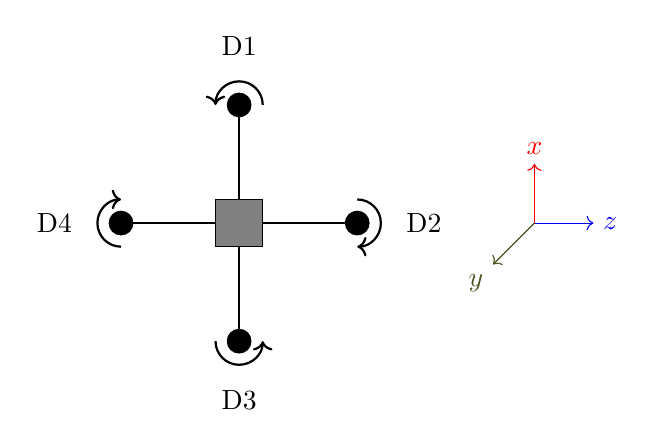
\begin{tikzpicture}[scale=1.5]
        % Coordinate system
        % \draw[->] (0,0) -- (1,0) node[right=1cm] {$z$};
        % \draw[->] (0,0) -- (0,1) node[above=1cm] {$x$};
        % \draw[->] (0,0) -- (-0.6,-0.6) node[below left] {$y$};
        
        % Quadrotor body
        \draw[fill=gray] (-0.2,0.2) rectangle (0.2,-0.2);
        
        % Arms
        \draw[thick] (-0.2,0) -- (-1,0);
        \draw[thick] (0.2,0) -- (1,0);
        \draw[thick] (0,0.2) -- (0,1);
        \draw[thick] (0,-0.2) -- (0,-1);

        % Axes
        \draw[->,red] (2.5,0) -- (2.5,0.5) node[above] {$x$};
        \draw[->,blue] (2.5,0) -- (3,0) node[right] {$z$};
        \draw[->,armygreen] (2.5,0) -- (2.15,-0.35) node[below left] {$y$};
        
        % Rotors with labels and direction
        % D1
        \draw[fill=black] (-1,0) circle (0.1) node[left=0.5cm] {D4};
        \draw[->,thick] (-1,-0.2) arc (270:90:0.2);
        % D2
        \draw[fill=black] (1,0) circle (0.1) node[right=0.5cm] {D2};
        \draw[->,thick] (1,0.2) arc (90:-90:0.2);
        % D3
        \draw[fill=black] (0,1) circle (0.1) node[above=0.5cm] {D1};
        \draw[->,thick] (0.2,1) arc (0:180:0.2);
        % D4
        \draw[fill=black] (0,-1) circle (0.1) node[below=0.5cm] {D3};
        \draw[->,thick] (-0.2,-1) arc (180:360:0.2);
    \end{tikzpicture}
    \caption{Quadcopter Body Diagram in the x-z plane}
    \label{fig:quadcopter}
\end{figure}

\begin{figure}[H]
    \centering
    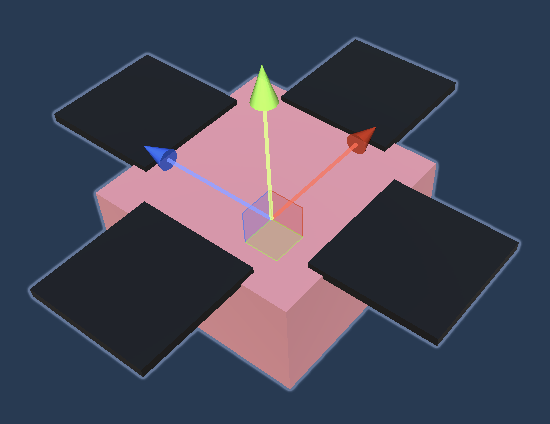
\includegraphics[height=80px]{agent}
    \caption{Agent in Unity}
    \label{fig:quadcopter-unity}
\end{figure}

For this investigation, a quadcopter was chosen as the type of agent, rather than a fixed-wing aircraft, due to increased maneouverability, simplicity when considering autonomous flight and simplicity in takeoff and landing procedures \cite{Thamm}.

There are four elements of control for an agent:
\begin{itemize}
    \item Roll angle (in radians), $\psi$
    \item Pitch angle (in radians), $\theta$
    \item Yaw rate (in $\frac{rad}{s}$), $\phi$
    \item Vertical thrust (in Newtons), $T$
\end{itemize}

We can define roll ($\psi$) as the rotation of the agent about the $x$ axis, pitch ($\theta$) as the rotation about the $z$ axis, and yaw ($\phi$) as the rotation about the $y$ axis.

For simplicity, these can be solely controlled by combinations of propeller thrust levels. 

A base thrust level, $T_b$, can be defined, which is the minimum thrust level required to maintain a stable hover. This is the thrust level required to counteract gravity, so $T_b = mg$. For each control operation, $T_b$ can be augmented by a thrust level, $T_{add}$, such that $|T_{add}| < T_b$, which is the additional thrust required to perform the operation.

As such, the control parameters can be operated by the following eight combinations of thrust levels for each propeller, with a high thrust level $T_{add} > 0$ and a low thrust level $T_{add} < 0$:


\begin{table}[H]
    \begin{center}
    \begin{tabular}{| c | c | c |} 
    \hline
    Operation & High Thrust & Low Thrust \\ 
    \hline
    Positive Roll, $\psi_+$ & $D_4$ & $D_2$ \\
    \hline
    Negative Roll, $\psi_-$ & $D_2$ & $D_4$ \\
    \hline
    Positive Pitch, $\theta_+$ & $D_3$ & $D_1$ \\
    \hline
    Negative Pitch, $\theta_-$ & $D_1$ & $D_3$ \\
    \hline
    Positive Thrust, $T_+$ & $D_1, D_2, D_3, D_4$ & none \\
    \hline
    Negative Thrust, $T_-$ & none & $D_1, D_2, D_3, D_4$ \\
    \hline
    \end{tabular}
    \end{center}
    \caption{Control Operations and Thrust Levels}
    \label{tab:control}
\end{table}


It is noted that yaw is omitted from Fig. \ref{tab:control}. For the purposes of the simulation, the propellers do not rotate. This lends itself to needing a workaround for simulating yaw. In \emph{Unity}'s physics engine, the rotation of opposite propellers can be simulated by applying forces along the $x$ and $z$ axes. As such, yaw is simulated according to the values in \ref{tab:yaw-control}.

\begin{table}[H]
    \begin{center}
    \begin{tabular}{| c | c | c |} 
    \hline
    Operation & Propeller & Direction of Force (respectively) \\ 
    \hline
    Positive Yaw, $\phi_+$ & $D_1, D_2$ & $Z_-, X_-$ \\
    \hline
    Positive Yaw, $\phi_+$ & $D_3, D_4$ & $Z_+, X_+$ \\
    \hline
    Negative Yaw, $\phi_-$ & $D_1, D_2$ & $Z_+, X_+$ \\
    \hline
    Negative Yaw, $\phi_-$ & $D_3, D_4$ & $Z_-, X_+$ \\
    \hline
    \end{tabular}
    \end{center}
    \caption{Yaw Directions and Respective Forces}
    \label{tab:yaw-control}
\end{table}

In real world physics, a couple of propellers could not provide thrust in both extremes of the same axes, as they could not switch rotation direction. Likewise, forces in adjacent propellers would not cause rotation in the same direction. However, for the purposes of simplicity within the simulation, this is ignored.

It is then possible to set some thrust constants for each control operation. An example assigment for the pitch and roll operations is seen below in Fig. \ref{tab:thrust-constants}.

\begin{table}[H]
    \begin{center}
    \begin{tabular}{| c | c | c |} 
    \hline
    Thrust Level & Thrust ($N$) \\ 
    \hline
    High & $\frac{2m \cdot g}{4}$\\
    \hline
    Normal & $\frac{m \cdot g}{4}$\\
    \hline
    Low & $\frac{0.5m \cdot g}{4}$\\
    \hline
    \end{tabular}
    \end{center}
    \caption{Thrust Constants for a drone of mass $m$ kg}
    \label{tab:thrust-constants}
\end{table}

At this stage, we have a model for the control and movement of the agent. An input is given to the propeller controller, which outputs the thrust level as required in Fig. \ref{tab:thrust-constants} to the individual propellers, causing a rotation of the agent in the desired direction.


\subsection{Stabilisation}
\label{sec:stabilisation}

An issue arises with this implementation; the simulation becomes unstable as thrust cannot be provided in an accurate enough manner to counteract excessive rotation, notably in the roll and pitch axes.

This can lead to the agent's rotation becoming overly large, causing it to roll over. If we consider an example input, represented by a single keypress to generate thrust to cause a pitch rotation, we can model the deviation from the desired pitch angle $\theta_{d} = 0.26$ over time, as shown in Fig. \ref{fig:pitch-angle}.

\begin{figure}[H]
\centering
\begin{tikzpicture}
    \begin{axis}[
        xlabel={Time, $t$ (s)},
        ylabel={Deviation from $\theta_d$ (rad)},
        ymajorgrids=true,
        grid style=dashed,
        y dir=reverse,
        xmax=4
    ]
    \draw[thin] (axis cs:\pgfkeysvalueof{/pgfplots/xmin},0) -- (axis cs:\pgfkeysvalueof{/pgfplots/xmax},0);
    
    \addplot[
        color=blue,
        mark=none,
        ]
        table[col sep=comma, x=x, y=y] {pitchAngle.csv};
        \legend{Your Data}
    
    \end{axis}
\end{tikzpicture}
\caption{Pitch angle due to input over time}
\label{fig:pitch-angle}
\end{figure}

Fig. \ref{fig:pitch-angle} shows that when given an input, the agent exceeds the desired pitch angle, crossing $\theta_d = 0$, then continues to rotate until it collides with the ground at $t = 3$ seconds.

As such, the need for a control system becomes apparent. 

\subsubsection{Proportional Controller}
A first intuition here is to control the rotation by reducing the thrust level as the agent approaches the desired angle, such that the thrust level at some time, $t$, is inversely proportional to the deviation from the desired angle as shown in Eq. \ref{eq:p-controller}.

\begin{equation}
    T_t \propto \frac{1}{\theta_d}
    \label{eq:p-controller}
\end{equation}

We can then define a proportionality constant, $K_p$ according to the inverse relationship in Eq. \ref{eq:p-controller}. Using different values for $K_p$, we can observe some behaviours in the deviation from the desired angle over time, as shown in Fig. \ref{fig:pitch-angle2}, which is split into two subfigures for clarity. The left-hand graph shows $K_p = 1$ and $K_p = 5$, and the right-hand graph shows $K_p = 5$ and $K_p = 10$.

\begin{figure}[H]
    \centering
    \begin{subfigure}{.4\textwidth}
    \begin{tikzpicture}[trim axis left, trim axis right]
        \begin{axis}[
            xlabel={Time, $t$ (s)},
            ylabel={Deviation from $\theta_d$ (rad)},
            ymajorgrids=true,
            grid style=dashed,
            y dir=reverse,
            xmax=9
        ]
        \draw[thin] (axis cs:\pgfkeysvalueof{/pgfplots/xmin},0) -- (axis cs:\pgfkeysvalueof{/pgfplots/xmax},0);
        
        \addplot[
            color=blue,
            mark=none,
            line width=0.5mm,
            ]
            table[col sep=comma, x=x, y=y] {pcontrol1.csv};

        \addplot[
            color=red,
            mark=none,
            ]
            table[col sep=comma, x=x, y=y] {pcontrol5.csv};

            % \addplot[
            %     color=green,
            %     mark=none,
            %     ]
            %     table[col sep=comma, x=x, y=y] {pcontrol10.csv};
        
            \addlegendentry{$K_p = 1$};
            \addlegendentry{$K_p = 5$};
        
        \end{axis}
    \end{tikzpicture}
\end{subfigure}
\hfill
\begin{subfigure}{.4\textwidth}
    \begin{tikzpicture}[trim axis left, trim axis right]
        \begin{axis}[
            xlabel={Time, $t$ (s)},
            ymajorgrids=true,
            grid style=dashed,
            y dir=reverse,
            xmax=9
        ]
        \draw[thin] (axis cs:\pgfkeysvalueof{/pgfplots/xmin},0) -- (axis cs:\pgfkeysvalueof{/pgfplots/xmax},0);
        
        % \addplot[
        %     color=blue,
        %     mark=none,
        %     ]
        %     table[col sep=comma, x=x, y=y] {pcontrol1.csv};

        \addplot[
            color=red,
            mark=none,
            line width=0.2mm,
            ]
            table[col sep=comma, x=x, y=y] {pcontrol5.csv};

            \addplot[
                color=purple,
                mark=none,
                line width=0.3mm
                ]
                table[col sep=comma, x=x, y=y] {pcontrol10.csv};
        
                \addlegendentry{$K_p = 5$};
                \addlegendentry{$K_p = 10$};
        
        \end{axis}
    \end{tikzpicture}
\end{subfigure}
    \caption{Pitch angle due to input over time with proportional error correction}
    \label{fig:pitch-angle2}
    \end{figure}

As shown in Fig. \ref{fig:pitch-angle2}, we can see that adding a proportional controller to the system creates a steady state, as we can see that the limit of $\theta_d$ as $t \to \infty$ is $\approx 0$ in both graphs.

In the left-hand graph, we can see that increasing $K_p$ decreases the amount of deviation from the desired angle. However, in the right-hand graph, we can see that this increase becomes negligible at a point, and does not reach zero. Instead, we can observe some oscillations in this state, as the agent continually overshoots the desired angle, before correcting itself, and overshooting again, to a lesser extent each time.

In some sense, we require the agent's controller to predict overshooting the desired angle.

\subsubsection{Derivative Controller}

In order to predict overshooting the desired angle, we need to modify the controller to consider the rate of change of the deviation. A deviation that is changing rapidly (oscillating) will also have a large (but decreasing) rate of change of deviation.

Hence, we can aim to reduce this rate of change of deviation by adding a term to the controller that is proportional to the rate of change of deviation, namely, a derivative term. This is shown in Eq. \ref{eq:pd-controller}.

\begin{equation}
    T_t \propto \frac{1}{\theta_d} - K_d \frac{d\theta}{dt}
    \label{eq:pd-controller}
\end{equation}

As before, we can introduce a proportionality constant, $K_d$, to the derivative term. We can then observe the effect of this term on the deviation from the desired angle over time, as shown in Fig. \ref{fig:pitch-angle3}. We note that we keep $K_p = 5$ constant.

\begin{figure}[H]
    \centering
    \begin{subfigure}{.4\textwidth}
        \begin{tikzpicture}[trim axis left, trim axis right]
            \begin{axis}[
                xlabel={Time, $t$ (s)},
                ylabel={Deviation from $\theta_d$ (rad)},
                ymajorgrids=true,
                grid style=dashed,
                y dir=reverse,
                xmax=2,
                ymax=0.14,
                ymin=-0.28
            ]
            \draw[thin] (axis cs:\pgfkeysvalueof{/pgfplots/xmin},0) -- (axis cs:\pgfkeysvalueof{/pgfplots/xmax},0);
            
            % \addplot[
            %     color=blue,
            %     mark=none,
            %     ]
            %     table[col sep=comma, x=x, y=y] {pcontrol1.csv};
    
            \addplot[
                color=red,
                mark=none,
                line width=0.2mm,
                ]
                table[col sep=comma, x=x, y=y] {pdcontrol1.csv};
    
                \addplot[
                    color=purple,
                    mark=none,
                    line width=0.3mm
                    ]
                    table[col sep=comma, x=x, y=y] {pdcontrol5.csv};
            
                    \addlegendentry{$K_p = 5,K_d = 0.1$};
                    \addlegendentry{$K_p = 5,K_d = 0.5$};  
            \end{axis}
        \end{tikzpicture}
    \end{subfigure}
    \hfill
    \begin{subfigure}{.4\textwidth}
        \begin{tikzpicture}[trim axis left, trim axis right]
            \begin{axis}[
                xlabel={Time, $t$ (s)},
                ymajorgrids=true,
                grid style=dashed,
                y dir=reverse,
                xmax=2,
                ymax=0.14,
                ymin=-0.28
            ]
            \draw[thin] (axis cs:\pgfkeysvalueof{/pgfplots/xmin},0) -- (axis cs:\pgfkeysvalueof{/pgfplots/xmax},0);
            
            % \addplot[
            %     color=blue,
            %     mark=none,
            %     ]
            %     table[col sep=comma, x=x, y=y] {pcontrol1.csv};
    
            \addplot[
                color=red,
                mark=none,
                line width=0.2mm,
                ]
                table[col sep=comma, x=x, y=y] {pdcontrol5.csv};
    
                \addplot[
                    color=purple,
                    mark=none,
                    line width=0.3mm
                    ]
                    table[col sep=comma, x=x, y=y] {pdcontrol20.csv};
            
                    \addlegendentry{$K_p = 5,K_d = 0.5$};
                    \addlegendentry{$K_p = 5,K_d = 1$};
            
            \end{axis}
        \end{tikzpicture}
    \end{subfigure}
    \caption{Pitch angle due to input over time with additional derivative error correction}
    \label{fig:pitch-angle3}
\end{figure}

Fig. \ref{fig:pitch-angle3} shows that adding a derivative controller with a small $K_d$ reduces the length of time of oscillation before reaching the desired angle. This behaviour can be seen at $K_d = 0.1$. At $K_d = 0.5$, this behaviour is improved and the oscillations stop entirely. However, at $K_d = 1$, whilst the controller achieves a steady state with minimal oscillation, it has overshot the desired angle, introducing steady state error into the system.

Furthermore, a second issue with the system has arisen; the agent's rotation is not quick enough to respond to an input. For example, we can see the responsiveness of the agent to a new input in Fig. \ref{fig:pitch-angle4}, where a forward pitch command is given, as before, at $t = 0$ seconds, then a backward pitch command is given at $t = 3.7$ seconds, both of which are shown as vertical lines on the graph.

We can see that the time to settle is $\approx 0.5$ seconds, which may cause issues in our simulation. When introducing multiple agents into the system, responsiveness is key, to ensure last minute direction changes can be made, for example, to avoid collisions.

\begin{figure}
    \centering
    \begin{tikzpicture}[trim axis left, trim axis right]
        \begin{axis}[
            xlabel={Time, $t$ (s)},
            ylabel={Deviation from $\theta_d$ (rad)},
            ymajorgrids=true,
            grid style=dashed,
            y dir=reverse,
            xmax=6,
            % ymax=0.14,
            % ymin=-0.28
        ]
        \draw[thin] (axis cs:\pgfkeysvalueof{/pgfplots/xmin},0) -- (axis cs:\pgfkeysvalueof{/pgfplots/xmax},0);

        \draw[thin] (axis cs:3.681287,\pgfkeysvalueof{/pgfplots/ymin}) -- (axis cs:3.681287,\pgfkeysvalueof{/pgfplots/ymax});

        \draw[thin] (axis cs:0,\pgfkeysvalueof{/pgfplots/ymin}) -- (axis cs:0,\pgfkeysvalueof{/pgfplots/ymax});
        
        % \addplot[
        %     color=blue,
        %     mark=none,
        %     ]
        %     table[col sep=comma, x=x, y=y] {pcontrol1.csv};

        \addplot[
            color=red,
            mark=none,
            line width=0.2mm,
            ]
            table[col sep=comma, x=x, y=y] {pdproblem.csv};

            % \addplot[
            %     color=purple,
            %     mark=none,
            %     line width=0.3mm
            %     ]
            %     table[col sep=comma, x=x, y=y] {pdcontrol20.csv};
        
                \addlegendentry{$K_p = 5,K_d = 0.5$};
                % \addlegendentry{$K_d = 1$};
        
        \end{axis}
    \end{tikzpicture}
    \caption{Pitch angle due to inputs at $t = 0$ and $t = 3.7$ seconds}
    \label{fig:pitch-angle4}
\end{figure}



\subsubsection{Integral Controller}
\label{sec:integral-controller}
We are able to reduce this reaction time and the possibility of steady state error by attempting to reduce the area between the $\theta_d$ and the actual angle (the curve in the graphs). 

Namely, we can introduce an integral term, which is proportional to the area between the $\theta_d$ and the actual angle. This is shown in Eq. \ref{eq:pid-controller}.

\begin{equation}
    T_t \propto \int_0^t \theta_d - \theta(\tau) d\tau
    \label{eq:pid-controller}
\end{equation}

We can then observe the effect of this term on the deviation from the desired angle over time, as shown in Fig. \ref{fig:pitch-angle5}. We note that we keep $K_p = 5$ and $K_d = 0.5$ constant, and test the values $K_i = 2$ and $K_i = 5$.

\begin{figure}[H]
    \centering
    \begin{subfigure}{.4\textwidth}
    \begin{tikzpicture}[trim axis left, trim axis right]
        \begin{axis}[
            xlabel={Time, $t$ (s)},
            ylabel={Deviation from $\theta_d$ (rad)},
            ymajorgrids=true,
            grid style=dashed,
            y dir=reverse,
            xmax=3,
            % ymax=0.14,
            % ymin=-0.28
        ]
        \draw[thin] (axis cs:\pgfkeysvalueof{/pgfplots/xmin},0) -- (axis cs:\pgfkeysvalueof{/pgfplots/xmax},0);

        \draw[thin] (axis cs:1.391017,\pgfkeysvalueof{/pgfplots/ymin}) -- (axis cs:1.391017,\pgfkeysvalueof{/pgfplots/ymax});

        \draw[thin] (axis cs:0,\pgfkeysvalueof{/pgfplots/ymin}) -- (axis cs:0,\pgfkeysvalueof{/pgfplots/ymax});
        
        % \addplot[
        %     color=blue,
        %     mark=none,
        %     ]
        %     table[col sep=comma, x=x, y=y] {pcontrol1.csv};

        \addplot[
            color=red,
            mark=none,
            line width=0.2mm,
            ]
            table[col sep=comma, x=x, y=y] {pidcontrol2.csv};

            % \addplot[
            %     color=purple,
            %     mark=none,
            %     line width=0.3mm
            %     ]
            %     table[col sep=comma, x=x, y=y] {pdcontrol20.csv};
        
                \addlegendentry{$K_p = 5,K_i=2,K_d = 0.5$};
                % \addlegendentry{$K_d = 1$};
        
        \end{axis}
    \end{tikzpicture}
\end{subfigure}
\hfill
\begin{subfigure}{.4\textwidth}
    \begin{tikzpicture}[trim axis left, trim axis right]
        \begin{axis}[
            xlabel={Time, $t$ (s)},
            ymajorgrids=true,
            grid style=dashed,
            y dir=reverse,
            xmax=3,
            % ymax=0.14,
            % ymin=-0.28
        ]
        \draw[thin] (axis cs:\pgfkeysvalueof{/pgfplots/xmin},0) -- (axis cs:\pgfkeysvalueof{/pgfplots/xmax},0);

        \draw[thin] (axis cs:1.391017,\pgfkeysvalueof{/pgfplots/ymin}) -- (axis cs:1.391017,\pgfkeysvalueof{/pgfplots/ymax});

        \draw[thin] (axis cs:0,\pgfkeysvalueof{/pgfplots/ymin}) -- (axis cs:0,\pgfkeysvalueof{/pgfplots/ymax});
        
        % \addplot[
        %     color=blue,
        %     mark=none,
        %     ]
        %     table[col sep=comma, x=x, y=y] {pcontrol1.csv};

        \addplot[
            color=red,
            mark=none,
            line width=0.2mm,
            ]
            table[col sep=comma, x=x, y=y] {pidcontrol5.csv};

            % \addplot[
            %     color=purple,
            %     mark=none,
            %     line width=0.3mm
            %     ]
            %     table[col sep=comma, x=x, y=y] {pdcontrol20.csv};
        
                \addlegendentry{$K_p = 5,K_i=5,K_d = 0.5$};
                % \addlegendentry{$K_d = 1$};
        
        \end{axis}
    \end{tikzpicture}
    \end{subfigure}
    \caption{Pitch angle due to inputs at $t = 0$ and $t = 1.4$ seconds}
    \label{fig:pitch-angle5}
\end{figure}

We note that the time to achieve a steady state is reduced, meaning the responsiveness of the system has improved. However, we note now that with the constant $K_p = 5, K_i = 5, K_d=0.5$, an overshoot is present. To mitigate this, we can increase $K_d$. This is shown in Fig. \ref{fig:pitch-angle6}.

\begin{figure}[H]
    \centering
    \begin{tikzpicture}[trim axis left, trim axis right]
        \begin{axis}[
            xlabel={Time, $t$ (s)},
            ylabel={Deviation from $\theta_d$ (rad)},
            ymajorgrids=true,
            grid style=dashed,
            y dir=reverse,
            xmax=3,
            % ymax=0.14,
            % ymin=-0.28
        ]
        \draw[thin] (axis cs:\pgfkeysvalueof{/pgfplots/xmin},0) -- (axis cs:\pgfkeysvalueof{/pgfplots/xmax},0);

        \draw[thin] (axis cs:1.63,\pgfkeysvalueof{/pgfplots/ymin}) -- (axis cs:1.63,\pgfkeysvalueof{/pgfplots/ymax});

        \draw[thin] (axis cs:0,\pgfkeysvalueof{/pgfplots/ymin}) -- (axis cs:0,\pgfkeysvalueof{/pgfplots/ymax});
        
        % \addplot[
        %     color=blue,
        %     mark=none,
        %     ]
        %     table[col sep=comma, x=x, y=y] {pcontrol1.csv};

        \addplot[
            color=red,
            mark=none,
            line width=0.2mm,
            ]
            table[col sep=comma, x=x, y=y] {pidmodified.csv};

            % \addplot[
            %     color=purple,
            %     mark=none,
            %     line width=0.3mm
            %     ]
            %     table[col sep=comma, x=x, y=y] {pdcontrol20.csv};
        
                \addlegendentry{$K_p = 5,K_i=5,K_d = 0.8$};
                % \addlegendentry{$K_d = 1$};
        
        \end{axis}
    \end{tikzpicture}
    \caption{Pitch angle due to inputs at $t = 0$ and $t = 1.6$ seconds}
    \label{fig:pitch-angle6}
\end{figure}

Note that in Fig. \ref{fig:pitch-angle6}, the overshoot is reduced, but we now have steady state and small angle oscillation errors. We can see that tuning the PID controller is a complex task akin to a chicken-and-egg problem, which we will explore further in Section \ref{sec:pid-tuning}.

\subsubsection{PID Controller}

We have constructed a PID (Proportional-Integral-Derivative) system; a feedback control system which uses the error between the current state and the desired state to calculate the control parameters. We now generalise this for all possible movement operations and call the desired state $r$ and the current state $y$.

Fig. \ref{fig:pid} shows the feedback loop of the PID controller. The error, $e(t)$, is calculated as the difference between the desired state, $r$, and the current state, $y$. The error is then fed into the three controllers. The output of each controller is then summed to produce the control variable, $u(t)$, which is then fed into the system. The system then produces the output, $y$, which is fed back into the error calculation.

\begin{figure}[H]
    \centering
    \tikzstyle{block} = [draw, fill=blue!20, rectangle, 
    minimum height=1em, minimum width=6em]
    \tikzstyle{sum} = [draw, fill=blue!20, circle, node distance=1cm]
    \tikzstyle{input} = [coordinate]
    \tikzstyle{output} = [coordinate]
    \tikzstyle{pinstyle} = [pin edge={to-,thin,black}]

    \begin{tikzpicture}[auto, node distance=2cm,>=latex']

    \node [input, name=input1] {};
    \node [sum, right of=input1] (sum) {$\Sigma$};
    \node [block, right of=sum, node distance=2.5cm] (I) {Integral};
    \node [block, above of=I, node distance=0.8cm] (P) {Proportional};
    \node [block, below of=I, node distance=0.8cm] (D) {Derivative};
    \node [sum, right of=I, node distance=2cm] (system) {$\Sigma$};
    \node [block, right of=system, node distance=2.5cm] (quad) {Quadcopter};
    \node [output, right of=quad] (output) {};

    \draw [draw,->] (input1) -- node {$r$} (sum);
    \draw [->] (sum) -- node {$e(t)$} (I);
    \draw [->] (sum) |- node {} (P.west);
    \draw [->] (sum) |- node {} (D.west);
    \draw [->] (I) -- node {} (system);
    \draw [->] (P) -| node {} (system);
    \draw [->] (D) -| node {} (system);
    \draw [->] (system) -- node {$u(t)$} (quad);
    \draw [->] (quad) -- node {$y$} (output);
    \draw [->] (quad.south) -- +(0,-1) -- +(-7.35,-1) -- node[] {-} (sum.200);
    \end{tikzpicture}
    \caption{PID Controller}
    \label{fig:pid}
\end{figure}


The PID controller is defined by three constant parameters derived earlier, $K_p$, $K_i$ and $K_d$, which are the proportional, integral and derivative gains respectively. The control variable, $u(t)$, is then defined as:

\begin{equation}
    u(t) = K_p e(t) + K_i \int_0^t e(\tau) d\tau + K_d \frac{de(t)}{dt}
\end{equation}


where $e(t)$ is the error at time $t$. Considering our simulation operates in discrete time intervals (frames), this can be approximated, using the \emph{Euler method} as:

\begin{equation}
    u(t) = K_p e(t) + K_i \frac{(e_t+e_{t-1})t}{2} + K_d \frac{e_t-e_{t-1}}{t}
\end{equation}

Hence, a feedback loop of the entire system can be produced, taking into account different PID controllers for each control operation. This is shown in Fig. \ref{fig:pid-feedback}.

\begin{figure}[H]
    \centering
    \tikzstyle{block} = [draw, fill=blue!20, rectangle, 
    minimum height=1em, minimum width=6em]
    \tikzstyle{sum} = [draw, fill=blue!20, circle, node distance=1cm]
    \tikzstyle{input} = [coordinate]
    \tikzstyle{output} = [coordinate]
    \tikzstyle{pinstyle} = [pin edge={to-,thin,black}]

    \begin{tikzpicture}[auto, node distance=1.3cm,>=latex']

    \node [input, name=altitude] {$T$};
    \node [input, name=pitch, below of=altitude] {$\theta$};
    \node [input, name=roll, below of=pitch] {$\psi$};
    \node [input, name=yaw, below of=roll] {$\phi$};

    \node [block, right of=altitude, node distance=2.5cm] (alt) {$PID_{altitude}$};
    \node [block, right of=pitch, node distance=2.5cm] (pt) {$PID_{pitch}$};
    \node [block, right of=roll, node distance=2.5cm] (rl) {$PID_{roll}$};
    \node [block, right of=yaw, node distance=2.5cm] (yw) {$PID_{yaw}$};


    \node [input, name=guide1, right of=pt, node distance=2.5cm] {};
    \node [input, name=guide2, right of=rl, node distance=2.5cm] {};

    \node [block] (output) at ($(guide1)!0.5!(guide2)$) {Quadcopter};

    \draw [->] (altitude) -- node {$T$} (alt);
    \draw [->] (pitch) -- node {$\theta$} (pt);
    \draw [->] (roll) -- node {$\psi$} (rl);
    \draw [->] (yaw) -- node {$\phi$} (yw);

    \draw [->] (alt.east) -| +(0.2,+0.4) -- +(-2.5,+0.4) |- node[] {} (alt.170);
    \draw [->] (pt.east) -| +(0.2,+0.4) -- +(-2.5,+0.4) |- node[] {} (pt.170);
    \draw [->] (rl.east) -| +(0.2,+0.4) -- +(-2.5,+0.4) |- node[] {} (rl.170);
    \draw [->] (yw.east) -| +(0.2,+0.4) -- +(-2.5,+0.4) |- node[] {} (yw.170);

    \draw [->] (alt.east) -| node {} (output);
    \draw [->] (pt.east) -| node {} (output);
    \draw [->] (rl.east) -| node {} (output);
    \draw [->] (yw.east) -| node {} (output);

    \end{tikzpicture}
    \caption{System Model}
    \label{fig:pid-feedback}
\end{figure}

\subsubsection{PID Parameter Tuning}
\label{sec:pid-tuning}
As noted previously in Section \ref{sec:integral-controller}, tuning the PID controller is a complex task and often suboptimal\cite{skogestad2001probably}. We require the PID controller to be stable, responsive and have minimal steady state error to ensure the agents are responsive and accurate in their movements.

\paragraph{Empirical Method}

Using a manual tuning method, we can observe the behaviour of the system and adjust the constants accordingly. A set of sufficient values were determined as shown in Fig. \ref{tab:pid-tuning}.

\begin{table}[H]
    \centering
        \begin{tabular}{| c | c | c | c |} 
        \hline
        Control Operation & $K_p$ & $K_i$ & $K_d$ \\ 
        \hline
        Thrust & 6 & 5 & 2 \\
        \hline
        Pitch & 10 & 10 & 2 \\
        \hline
        Roll & 10 & 10 & 2 \\
        \hline
        Yaw & 10 & 10 & 2 \\
        \hline
        \end{tabular}
        \caption{Tuning Constants}
        \label{tab:pid-tuning}
\end{table}

It is noted that the agent is slightly unstable at very small angles. This is negligible.

\paragraph{Ziegler-Nichols Method}
The Ziegler-Nichols method is a heuristic method for tuning PID controllers. It is based on the response of the system to a step input.

\citet{McCormack} propose a set of tuning rules for a classic control system, which result in the proportional gain $K_p$ and two values representing the integral and derivative time constants, $T_i,T_d$, respectively. An extract from \emph{Table 1} of the paper is shown in Table \ref{tab:zn}.

\begin{table}[h]
    \centering
    \begin{tabular}{c|c|c}
        \hline
        Tuning Rule & Required & Controller Parameters \\
        \hline
        ZN & \(K_u, T_u\) & \(K_p = 0.6K_u, T_i = 0.5T_u, T_d = 0.125T_u\) \\
        \hline
    \end{tabular}
    \caption{Ziegler-Nichols Method}
    \label{tab:zn}
\end{table}

The term $K_u$ refers to the optimal gain; the gain at which the system oscillates at a constant amplitude and frequency. The term $T_u$ refers to the time period of this oscillation.

Fig. \ref{fig:zn-tuning} shows the oscillation of the system following a positive pitch command with $K_p$ increasing from 1 at a rate of 1 every second. We can then determine the opimal gain to be the point at which the oscillations become stable. This is shown to be circa $K_p = 7$. A zoomed in version of the plot shows the time period of this oscillation to be $\approx T_u = 0.6$ seconds.


\begin{figure}[H]
    \centering
    \begin{subfigure}{.4\textwidth}
    \begin{tikzpicture}[trim axis left, trim axis right]
        \begin{axis}[
            xlabel={Time, $t$ (s) and $K_p$},
            ylabel={Deviation from $\theta_d$ (rad)},
            ymajorgrids=true,
            grid style=dashed,
            y dir=reverse,
            xmax=15,
            % ymax=0.14,
            ymin=-1
        ]
        % \draw[thin] (axis cs:\pgfkeysvalueof{/pgfplots/xmin},0) -- (axis cs:\pgfkeysvalueof{/pgfplots/xmax},0);

        \draw[thin] (axis cs:7,\pgfkeysvalueof{/pgfplots/ymin}) -- (axis cs:7,\pgfkeysvalueof{/pgfplots/ymax});

        % \draw[thin] (axis cs:0,\pgfkeysvalueof{/pgfplots/ymin}) -- (axis cs:0,\pgfkeysvalueof{/pgfplots/ymax});
        
        % \addplot[
        %     color=blue,
        %     mark=none,
        %     ]
        %     table[col sep=comma, x=x, y=y] {pcontrol1.csv};

        \addplot[
            color=red,
            mark=none,
            line width=0.2mm,
            ]
            table[col sep=comma, x=x, y=y] {pidtuningzn.csv};

            % \addplot[
            %     color=purple,
            %     mark=none,
            %     line width=0.3mm
            %     ]
            %     table[col sep=comma, x=x, y=y] {pdcontrol20.csv};
        
                % \addlegendentry{$K_p$};
                % \addlegendentry{$K_d = 1$};
        
        \end{axis}
    \end{tikzpicture}
\end{subfigure}
\hfill
\begin{subfigure}{.4\textwidth}
    \begin{tikzpicture}[trim axis left, trim axis right]
        \begin{axis}[
            xlabel={Time, $t$ (s) and $K_p$},
            % ylabel={Deviation from $\theta_d$ (rad)},
            ymajorgrids=true,
            grid style=dashed,
            y dir=reverse,
            xmax=9,
            xmin=7,
            % ymax=0.14,
            ymin=-1
        ]
        % \draw[thin] (axis cs:\pgfkeysvalueof{/pgfplots/xmin},0) -- (axis cs:\pgfkeysvalueof{/pgfplots/xmax},0);

        \draw[thin] (axis cs:7,\pgfkeysvalueof{/pgfplots/ymin}) -- (axis cs:7,\pgfkeysvalueof{/pgfplots/ymax});

        % \draw[thin] (axis cs:0,\pgfkeysvalueof{/pgfplots/ymin}) -- (axis cs:0,\pgfkeysvalueof{/pgfplots/ymax});
        
        % \addplot[
        %     color=blue,
        %     mark=none,
        %     ]
        %     table[col sep=comma, x=x, y=y] {pcontrol1.csv};

        \addplot[
            color=red,
            mark=none,
            line width=0.2mm,
            ]
            table[col sep=comma, x=x, y=y] {pidtuningzn.csv};

            % \addplot[
            %     color=purple,
            %     mark=none,
            %     line width=0.3mm
            %     ]
            %     table[col sep=comma, x=x, y=y] {pdcontrol20.csv};
        
                % \addlegendentry{$K_p$};
                % \addlegendentry{$K_d = 1$};
        
        \end{axis}
    \end{tikzpicture}
\end{subfigure}
    \caption{Oscillation of the system with varying $K_p$}
    \label{fig:zn-tuning}
\end{figure}

We can then use Table \ref{tab:zn} to determine the controller parameters. We find that $K_p = 4.2, T_i = 0.3, T_d = 0.075$.

At this stage, we can determine the values for the integral and derivative gains from the method, which states the relationships shown in Equation \ref{eq:pid-tuning-relationships}.

\begin{equation}
    \label{eq:pid-tuning-relationships}
    K_i = \frac{K_p}{T_i}
    \quad \text{and} \quad
    K_d = K_pT_d
\end{equation}

Hence, we find that $K_i = 14, K_d = 0.315$.

We can compare this behaviour with the values obtained from the empirical method described earlier. When given a positive pitch command to obtain the desired angle $\theta_d = 0.26$ radians, then a release of this command to reset the desired angle to $\theta_d = 0$, we can observe and compare the behaviours for both sets of constants. This is shown in Fig. \ref{fig:tuning-comparison}.

\begin{figure}
    \centering
    \begin{tikzpicture}[trim axis left, trim axis right]
        \begin{axis}[
            xlabel={Time, $t$ (s)},
            ylabel={Deviation from $\theta_d$ (rad)},
            ymajorgrids=true,
            grid style=dashed,
            y dir=reverse,
            xmax=4.5,
            width=\columnwidth,
            height=0.5\columnwidth
            % ymax=0.14,
            % ymin=-0.28
        ]
        \draw[thin] (axis cs:\pgfkeysvalueof{/pgfplots/xmin},0) -- (axis cs:\pgfkeysvalueof{/pgfplots/xmax},0);

        \draw[thin] (axis cs:2.04,\pgfkeysvalueof{/pgfplots/ymin}) -- (axis cs:2.04,\pgfkeysvalueof{/pgfplots/ymax});
        
        % \addplot[
        %     color=blue,
        %     mark=none,
        %     ]
        %     table[col sep=comma, x=x, y=y] {pcontrol1.csv};

        \addplot[
            color=red,
            mark=none,
            line width=0.2mm,
            ]
            table[col sep=comma, x=x, y=y] {znresults.csv};

            \addplot[
                color=blue,
                mark=none,
                line width=0.2mm
                ]
                table[col sep=comma, x=x, y=y] {empresults.csv};
        
                \addlegendentry{ZN: $K_p = 4.2, K_i = 14, K_d = 0.315$};
                \addlegendentry{Empirical: $K_p = 10, K_i = 10, K_d = 2$};
        
        \end{axis}
    \end{tikzpicture}
    \caption{Pitch angle due to inputs at $t = 0$ and $t = 2.03$ seconds}
    \label{fig:tuning-comparison}
\end{figure}

We can see that the empirical method results in a faster settling time, but has a small steady state error, which is not present in the results of the Ziegler-Nichols method. However, the Ziegler-Nichols method results in a small oscillation centered at the desired angle. 

As the Ziegler-Nichols method is a heuristic method, it is not guaranteed to be optimal. However, it is a good starting point for tuning the PID controller. We can see from our comparison that an ideal set of constants lies somewhere between the results from both methods. We can improve on our current results by observing the behaviour of the system and adjusting the constants accordingly.

Namely, we can see that the small oscillation present in the Ziegler-Nichols method can be reduced by increasing the derivative gain, such that $K_d = 0.9$. This should also mitigate the small steady-state error present from the empirical method. To reduce this further, we will adjust the proportional gain such that $K_p = 8$ and the integral gain such that $K_i = 12$.


This is shown in Fig. \ref{fig:combined-znemp}.

\begin{figure}[H]
    \centering
    \begin{tikzpicture}[trim axis left, trim axis right]
        \begin{axis}[
            xlabel={Time, $t$ (s)},
            ylabel={Deviation from $\theta_d$ (rad)},
            ymajorgrids=true,
            grid style=dashed,
            y dir=reverse,
            xmax=5,
            % ymax=0.14,
            % ymin=-0.28
        ]
        \draw[thin] (axis cs:\pgfkeysvalueof{/pgfplots/xmin},0) -- (axis cs:\pgfkeysvalueof{/pgfplots/xmax},0);

        \draw[thin] (axis cs:2.404,\pgfkeysvalueof{/pgfplots/ymin}) -- (axis cs:2.404,\pgfkeysvalueof{/pgfplots/ymax});

        % \addplot[
        %     color=blue,
        %     mark=none,
        %     ]
        %     table[col sep=comma, x=x, y=y] {pcontrol1.csv};

        \addplot[
            color=red,
            mark=none,
            line width=0.2mm,
            ]
            table[col sep=comma, x=x, y=y] {znempresults.csv};

            % \addplot[
            %     color=purple,
            %     mark=none,
            %     line width=0.3mm
            %     ]
            %     table[col sep=comma, x=x, y=y] {pdcontrol20.csv};
        
                \addlegendentry{$K_p = 8,K_i=12,K_d = 0.9$};
                % \addlegendentry{$K_d = 1$};
        
        \end{axis}
    \end{tikzpicture}
    \caption{Pitch angle due to inputs at $t = 0$ and $t = 1.6$ seconds}
    \label{fig:combined-znemp}
\end{figure}


\paragraph{Conclusion}
Fig. \ref{fig:combined-znemp} shows a tuned PID pitch controller, derived from a combination of empirical and heuristic methods. We will then extend these values to our other control operations, roll and yaw, and keep the thrust constants that we obtained through the empirical method for simplicity.

The final PID constants are shown in Table \ref{tab:pid-final}.

\begin{table}[H]
    \centering
        \begin{tabular}{| c | c | c | c |} 
        \hline
        Control Operation & $K_p$ & $K_i$ & $K_d$ \\ 
        \hline
        Thrust & 6 & 5 & 2 \\
        \hline
        Pitch & 8 & 12 & 0.9 \\
        \hline
        Roll & 8 & 12 & 0.9 \\
        \hline
        Yaw & 8 & 12 & 0.9 \\
        \hline
        \end{tabular}
        \caption{Final PID Constants}
        \label{tab:pid-final}
\end{table}

However, steady-state error is still present in the system. We can continue to use advanced methods to attempt to tune this, however, for the purposes of this project, we will consider this to be sufficient.

As such, we have completed our design of the agent physics model.

\subsection{Environment Model}
We will now discuss how the agents interact with each other and objects in the environment according to the Unity physics engine.

Agents may collide with any object in the environment defined to have a `collider'. This is a built-in Unity component that defines the shape of the object and is used to detect collisions. The agent's collider is comprised of the colliders of its parts, namely the agent's body and its rotors.

Likewise, all objects we instanitate from this point onwards, such as the terrain, obstacles and platforms, will have colliders.

We will specify that the agents are resistant to collisions with other agents.

\newpage
\section{Introducing Autonomy}
The initial aim is to achieve position control for an agent, such that when given a current position $p_0 = [x_0,y_0,z_0]$ and a goal position $p_{goal} = [x_1,y_1,z_1]$, the agent will move to the goal position. This sets the foundation for the behaviour of the agents; we will model these as a 'desire' to move to a specific position.

There are several methods for this. An agent may yaw to face the goal, then pitch towards it. In the case of this project, time-sensitive position decisions will need to be made when considering swarm dynamics and collision avoidance, so a more efficient method is required. As such, the aim will be to pitch and roll towards the position.

\subsection{Movement to Position}
We can determine the input commands required for an agent to reach $p_{goal}$ from $p_0$ by performing vector calculations. 

Firstly, we can model these two points on a coordinate grid. For representational clarity, we will assume the model to be in two dimensions for now. We can then calculate the vector between the two points, $v_g = p_{goal} - p_0$. We can see that the vector subtraction represents the transformation vector required to reach the goal position.

This is shown in Fig. \ref{fig:2d-coords}.

\begin{figure}[H]
    \centering
    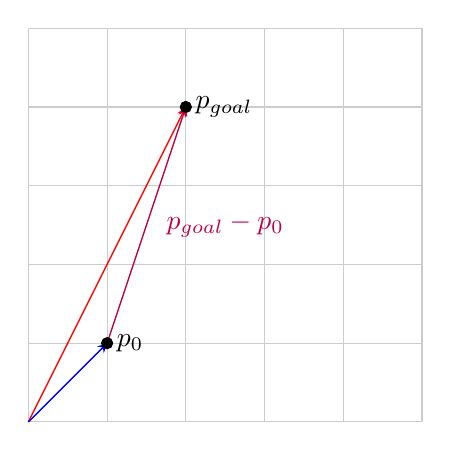
\begin{tikzpicture}
        \draw[thin,gray!40] (0,0) grid (5,5);
        % \draw[<->] (-8,0)--(2,0) node[right]{$x$};
        % \draw[<->] (0,-2)--(0,2) node[above]{$y$};
        % \draw[line width=2pt,blue,-stealth](0,0)--(1,1) node[anchor=south west]{$u$};
        \draw[line width=0.5pt,red,-stealth](0,0)--(2,4) node[anchor=north east]{};
        \draw[line width=0.5pt,blue,-stealth](0,0)--(1,1) node[anchor=north east]{};
        \draw[line width=0.5pt,purple,-stealth](1,1)--(2,4) node at (2.5,2.5){$p_{goal}-p_0$};
        \filldraw[black] (2,4) circle (2pt) node[anchor=west]{$p_{goal}$};
        \filldraw[black] (1,1) circle (2pt) node[anchor=west]{$p_{0}$};
      \end{tikzpicture}
    \caption{2D Coordinate Grid with $p_{goal}$ and $p_{0}$}
    \label{fig:2d-coords}
\end{figure}

We then require the agent to pitch and roll towards the goal position. This requires a change of basis between the global frame (as represented in \ref{fig:2d-coords}) and the agent's local frame. This is because the agent's yaw component means that the agent's pitch and roll directions will not cause a movement along the global axes, except the trivial case, where the agent is lined up with the global axes.

We can determine the transformation required to convert the global vector $v_g$ into the local frame, resulting in the vector $v_l$ by calculating the rotation matrix between the two frames of reference.

We can initially do this in two dimensions by determining a transformation matrix $M_2$ such that:

\begin{equation}
    \begin{bmatrix}
    x_l \\
    y_l
    \end{bmatrix}
    = M_2 \cdot
    \begin{bmatrix}
    x_g \\
    y_g
    \end{bmatrix}
\label{eq:basis-transformation2}
\end{equation}

We note that in the two-dimensional case, $M_2$ need only be a roation matrix representing the yaw of the agent. We can derive $M_2$ as follows. We first consider a vector in the global frame, $v_g$ and the local frame $v_l$. We note that their magnitudes are equal, with $|v_g| = |v_l|$. We can then determine the angle between the two vectors, $\beta$, and the angle between the global x-axis and the vector $v_g$, $\alpha$.

This is shown in Fig. \ref{fig:2d-rotation}.

\begin{figure}[H]
    \centering
    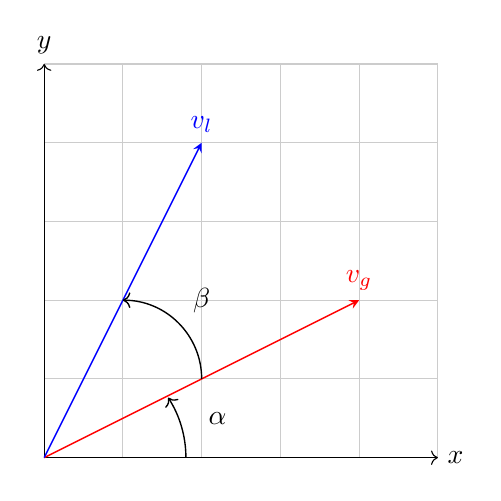
\begin{tikzpicture}
        \draw[thin,gray!40] (0,0) grid (5,5);
        \draw[->] (0,0)--(5,0) node[right]{$x$};
        \draw[->] (0,0)--(0,5) node[above]{$y$};
        % \draw[line width=2pt,blue,-stealth](0,0)--(1,1) node[anchor=south west]{$u$};
        \draw[line width=0.5pt,red,-stealth](0,0)--(4,2) node[above]{$v_g$};
        \draw[line width=0.5pt,blue,-stealth](0,0)--(2,4) node[above]{$v_l$};
        \draw[->,line width=0.5pt] (2,1) arc [start angle=0, end angle=90, radius=1] node at (2,2) {$\beta$};
        \draw[->,line width=0.5pt] (1.8,0) arc [start angle=0, end angle=33, radius=1.4] node at (2.2,0.5) {$\alpha$};
      \end{tikzpicture}
    \caption{2D Coordinate Grid with $v_l$ and $v_g$}
    \label{fig:2d-rotation}
\end{figure}

Hence, we can determine that the $x$ and $y$ components of $v_g$ are:

\begin{equation}
    \begin{aligned}
        x_g &= |v_g| \cos(\alpha) \\
        y_g &= |v_g| \sin(\alpha)
    \end{aligned}
\end{equation}

It must then hold that:

\begin{equation}
    \begin{aligned}
        x_l &= |v_l| \cos(\alpha + \beta) \\
        y_l &= |v_l| \sin(\alpha + \beta) \\
            &\implies \\
        x_l &= |v_g| \cos(\alpha)\cos(\beta) - |v_g| \sin(\alpha)\sin(\beta) \\
        y_l &= |v_g| \sin(\alpha)\cos(\beta) + |v_g| \cos(\alpha)\sin(\beta)
        \\
            &\implies \\
        x_l &= x_g \cos(\beta) - y_g \sin(\beta) \\
        y_l &= x_g \sin(\beta) + y_g \cos(\beta)
    \end{aligned}
\end{equation}

We can represent this as a matrix equation:
\begin{equation}
    \begin{bmatrix}
    x_l \\
    y_l
    \end{bmatrix}
    = 
    \begin{bmatrix}
    \cos(\beta) & -\sin(\beta) \\
    \sin(\beta) & \cos(\beta)
    \end{bmatrix}
    \begin{bmatrix}
    x_g \\
    y_g
    \end{bmatrix}
    \\ \text{, where } \\
    M_2 = 
    \begin{bmatrix}
    \cos(\beta) & -\sin(\beta) \\
    \sin(\beta) & \cos(\beta)
    \end{bmatrix}
\end{equation}

Returning to three dimensions, we can represent our problem as determining a transformation matrix $M_3$, such that:

\begin{equation}
   \begin{bmatrix}
    x_l \\
    y_l \\
    z_l
    \end{bmatrix}
    = M_3 \cdot
    \begin{bmatrix}
    x_g \\
    y_g \\
    z_g
    \end{bmatrix}
\label{eq:basis-transformation}
\end{equation}

In the three-dimensional case, $M_3$ will be a rotation matrix representing the yaw, pitch and roll of the agent. As such, it will be comprised of three individual rotation matrices for each axis of rotation. Hence:

\begin{equation}
    M_3 = R_y \cdot R_x \cdot R_z
\end{equation}

We can then derive the rotation matrix $R_x$ in a similar method to $M_2$.

We note that $R_x$ will represent a rotation about the x-axis, namely, the roll of the agent. This means that the $y$ and $z$ components of the vector $v_g$ will be rotated through an angle of $\psi$, whilst the $x$ component will remain constant. We can then determine the rotation matrix from earlier intuition as:

\begin{equation}
    R_x =
    \begin{bmatrix}
        1 & 0 & 0 \\
        0 & \cos(\psi) & -\sin(\psi) \\
        0 & \sin(\psi) & \cos(\psi)
    \end{bmatrix}
\end{equation}

Considering the other two rotation matrices, $R_y$ and $R_z$, where the $xz$ and $xy$ planes are rotated respectively, we can see:

\begin{equation}
    \begin{aligned}
        R_y &=
        \begin{bmatrix}
        \cos(\theta) & 0 & -\sin(\theta) \\
        0 & 1 & 0 \\
        \sin(\theta) & 0 & \cos(\theta)
        \end{bmatrix}
        \\
        R_z &=
        \begin{bmatrix}
        \cos(\phi) & \sin(\phi) & 0 \\
        -\sin(\phi) & \cos(\phi) & 0 \\
        0 & 0 & 1
        \end{bmatrix} 
    \end{aligned}
\end{equation}

At this stage, we can split the local vector $v_l$ into its constituent pitch and roll components, which can be applied to the agent as input commands.

We see that we may obtain the pitch and roll components of the vector $v_l$ by taking the $x$ and $z$ components respectively. This is shown in Fig. \ref{fig:pitch-roll}. 

\begin{figure}[H]
    \centering
    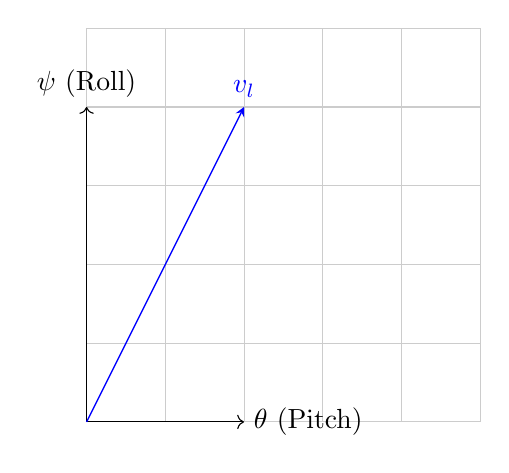
\begin{tikzpicture}
        \draw[thin,gray!40] (0,0) grid (5,5);
        \draw[->] (0,0)--(2,0) node[right]{$\theta$ (Pitch)};
        \draw[->] (0,0)--(0,4) node[above]{$\psi$ (Roll)};
        % \draw[line width=2pt,blue,-stealth](0,0)--(1,1) node[anchor=south west]{$u$};
        % \draw[line width=0.5pt,red,-stealth](0,0)--(4,2) node[above]{$v_g$};
        \draw[line width=0.5pt,blue,-stealth](0,0)--(2,4) node[above]{$v_l$};
        % \draw[->,line width=0.5pt] (2,1) arc [start angle=0, end angle=90, radius=1] node at (2,2) {$\beta$};
        % \draw[->,line width=0.5pt] (1.8,0) arc [start angle=0, end angle=33, radius=1.4] node at (2.2,0.5) {$\alpha$};
      \end{tikzpicture}
    \caption{Constituent Pitch and Roll Components of $v_l$}
    \label{fig:pitch-roll}
\end{figure}

Usefully, this conversion step can be performed in the Unity physics engine using the built-in method \verb|transform.InverseTransformVector()|, which will convert the vector from the global frame to the local frame of the agent.

% For the purposes of foreign obejcts in the simulation, namely terrain and obstacles, we will simulate the agents as having a light ranging device, namely LiDAR, which can detect the distance to the nearest object in a given direction. The \emph{Unity} physics engine has a built-in method for this, \verb|Physics.Raycast()|. This returns the distance to the nearest object in a given direction, or \verb|Infinity| if no object is detected. Whilst this is a significant abstraction of the real world implementation of a LiDAR sensor, it is sufficient for the purposes of this simulation. We go into more detail on the implementation of this in Section \ref{sec:terrain-avoidance}.


\subsection{Boids (1987)}
At this stage, we introduce multiple agents into the environment. We will initially consider the agents to be autonomous, and have the ability to hover by default.

We will make some assumptions about the awareness of the agents at this stage and provide some important definitions.
These are:
\begin{itemize}
    \item Agents are aware of the positions of all other agents within a certain radius, $r$. This is defined as the \emph{neighbourhood radius}.
    \item Agents are aware of their own position with respect to the global reference frame.
    \item Agents in a flock of size $n$ are defined as $a_1,...,a_n \in A$.
\end{itemize}

The motivation behind the use of the neighbourhood radius is to reduce computational complexity. Generally, an increase in the number of adjacent agents will result in an increase in the number of calculations required. We can reduce this by not including the agents that have no effect on the behaviour of the agent in question.

We will then introduce the concept of \emph{Boids} \cite{Reynolds}. This is a method of simulating flock behaviour, where agents are programmed to exhibit a set of behaviours that result in emergent flock behaviour. We will explore the implementation of these behaviours in the next section.

For all behaviours, we calculate a force vector that is applied to the agent, with respect to the agent's local frame.

\subsubsection{Avoidance}

The avoidance behaviour is used as a method for agents to avoid collisions with each other. To this end, the behaviour causes agents to move away from each other when they are within a certain distance of each other. 

We will call this distance $d$, and define it as the \emph{square avoidance radius}. This is the distance at which agents will begin to move away from each other. We will define this as the square of the distance between two agents, $a_1,a_2 \in A$, such that $d = (|a_1|-|a_2|)^2$, for the purposes of algorithmic efficiency. This is a common method in the \emph{Unity} physics engine \cite{unity}.

We can then determine the avoidance vector for an agent, $a$, by calculating the mean distance vector between $a$ and all other agents within the neighbourhood, $a_i$, such that $|a_i| - |a| < d$.

Specifically, we populate the set $R_a$ with all agents $a \in A$ that are within the neighbourhood of $a$.

\begin{equation}
\vec{A} = 
\begin{cases}
    0 & \text{if } R_a = \emptyset \\
    \frac{1}{|R_a|} \sum_{a_i \in R_a} \vec{a_i} - \vec{a} & \text{otherwise}
\end{cases}
\end{equation}

We can model an example with two agents in two-dimensional space. This can be seen in Fig. \ref{fig:avoidance-2d}. We see the two agents $a_1$ and $a_2$ have position vectors $[2,2]$ and $[3,3]$ respectively.

Hence, the avoidance vectors for the two agents are:
\begin{equation}
    \begin{aligned}
        \vec{a_{avoid}^1} &= \frac{1}{1} \left( \begin{bmatrix} 3 \\ 3 \end{bmatrix} - \begin{bmatrix} 2 \\ 2 \end{bmatrix} \right) = \begin{bmatrix} 1 \\ 1 \end{bmatrix} \\
        \vec{a_{avoid}^2} &= \frac{1}{1} \left( \begin{bmatrix} 2 \\ 2 \end{bmatrix} - \begin{bmatrix} 3 \\ 3 \end{bmatrix} \right) = \begin{bmatrix} -1 \\ -1 \end{bmatrix}
    \end{aligned}
\end{equation}

\begin{figure}[H]
    \centering
    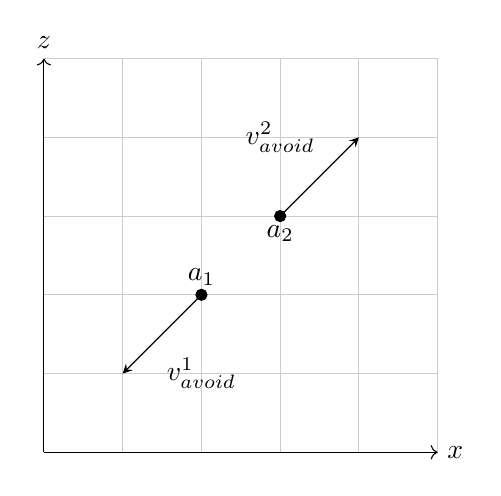
\begin{tikzpicture}
        \draw[thin,gray!40] (0,0) grid (5,5);
        \draw[->] (0,0)--(5,0) node[right]{$x$};
        \draw[->] (0,0)--(0,5) node[above]{$z$};

        \filldraw[black] (2,2) circle (2pt) node[anchor=south]{$a_1$};
        \filldraw[black] (3,3) circle (2pt) node[anchor=north]{$a_2$};

        \draw[line width=0.5pt,black,-stealth](2,2)--(1,1) node at (2,1){$v_{avoid}^1$};
        \draw[line width=0.5pt,black,-stealth](3,3)--(4,4) node at (3,4){$v_{avoid}^2$};
        
      \end{tikzpicture}
    \caption{Avoidance vectors for two nearby agents}
    \label{fig:avoidance-2d}
\end{figure}


\subsubsection{Alignment}

The alignment behaviour causes agents to align their headings with those of their neighbours. This may, in turn, reduce collisions. We can determine the alignment vector for an agent, $a$, by calculating the mean heading vector between $a$ and all other agents within the neighbourhood, $a_i$, such that $|a_i| - |a| < r$.

Specifically, we have:

\begin{equation}
\vec{B} =
\begin{cases}
    0 & \text{if } R_b = \emptyset \\
    \frac{1}{|R_b|} \sum_{a_i \in R_b} \vec{h(a_i)} & \text{otherwise}
\end{cases}
\end{equation}

We can model three agents in two-dimensional space. This can be seen in Fig. \ref{fig:alignment-2d}. We see the three agents $a_1$, $a_2$ and $a_3$ have heading vectors $[1,1]$, $[1,0]$ and $[0,1]$ respectively.

We introduce three agents as the simplest stable state of the system. Using only two agents would result in a system where the heading vectors would oscillate between the two agents without any external forces.

We can then determine the alignment vectors for the three agents as follows:

\begin{equation}
    \begin{aligned}
        \vec{a_{align}^1} &= \frac{1}{2} \left( \begin{bmatrix} 1 \\ 0 \end{bmatrix} + \begin{bmatrix} 0 \\ 1 \end{bmatrix} \right) = \begin{bmatrix} 0.5 \\ 0.5 \end{bmatrix} \\
        \vec{a_{align}^2} &= \frac{1}{2} \left( \begin{bmatrix} 1 \\ 1 \end{bmatrix} + \begin{bmatrix} 0 \\ 1 \end{bmatrix} \right) = \begin{bmatrix} 0.5 \\ 1 \end{bmatrix} \\
        \vec{a_{align}^3} &= \frac{1}{2} \left( \begin{bmatrix} 1 \\ 1 \end{bmatrix} + \begin{bmatrix} 1 \\ 0 \end{bmatrix} \right) = \begin{bmatrix} 1 \\ 0.5 \end{bmatrix}
    \end{aligned}
\end{equation}

We can visualise the current heading vectors at time $t$ and the determined heading vectors for time $t+1$ (indicated in red) in Fig. \ref{fig:alignment-2d}\footnote{N.B. The agents will likely not be in the same position after one timestep. We consider this as negligible in the visualisation.}, where we see the new heading vectors have less variance in their angles.

\begin{figure}[H]
    \centering
    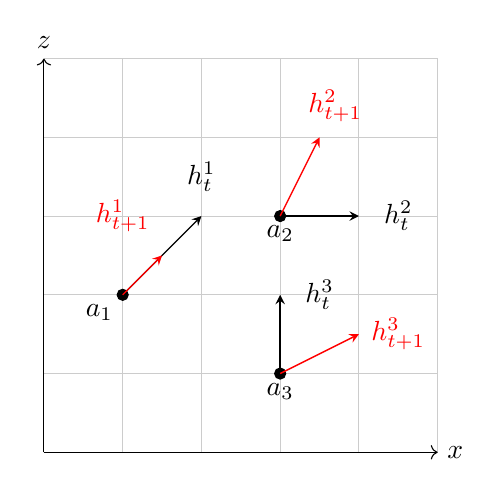
\begin{tikzpicture}
        \draw[thin,gray!40] (0,0) grid (5,5);
        \draw[->] (0,0)--(5,0) node[right]{$x$};
        \draw[->] (0,0)--(0,5) node[above]{$z$};

        \filldraw[black] (1,2) circle (2pt) node[anchor=north east]{$a_1$};
        \filldraw[black] (3,3) circle (2pt) node[anchor=north]{$a_2$};
        \filldraw[black] (3,1) circle (2pt) node[anchor=north]{$a_3$};

        \draw[line width=0.5pt,black,-stealth](1,2)--(2,3) node at (2,3.5){$h^1_t$};
        \draw[line width=0.5pt,black,-stealth](3,3)--(4,3) node at (4.5,3){$h^2_t$};
        \draw[line width=0.5pt,black,-stealth](3,1)--(3,2) node at (3.5,2){$h^3_t$};

        \draw[line width=0.5pt,red,-stealth](1,2)--(1.5,2.5) node at (1,3){$h^1_{t+1}$};
        \draw[line width=0.5pt,red,-stealth](3,3)--(3.5,4) node at (3.7,4.4){$h^2_{t+1}$};
        \draw[line width=0.5pt,red,-stealth](3,1)--(4,1.5) node at (4.5,1.5){$h^3_{t+1}$};
        
      \end{tikzpicture}
    \caption{Alignment vectors for three nearby agents}
    \label{fig:alignment-2d}
\end{figure}


\subsubsection{Cohesion}

Finally, we implement the third principle, \emph{cohesion}. This is in principle, the inverse to the avoidance principle. It ensure members of the flock stay together. We can determine the cohesion vector for an agent, $a$, by calculating the mean position vector between $a$ and all other agents within the neighbourhood, $a_i$, such that $|a_i| - |a| < r$.

Specifically, we have:

\begin{equation}
\vec{C} =
\begin{cases}
    0 & \text{if } R_c = \emptyset \\
    \left(
    \frac{1}{|R_c|} \sum_{a_i \in R_c} \vec{a_i} \right) - \vec{a} & \text{otherwise}
\end{cases}
\end{equation}

We consider three agents $a_1$, $a_2$ and $a_3$ in two-dimensional space with position vectors $[1,2]$, $[3,3]$ and $[3,1]$ respectively. We can then determine the cohesion vectors for the three agents as follows:

\begin{equation}
    \begin{aligned}
        \vec{a_{cohere}^1} &= \frac{1}{2} \left( \begin{bmatrix} 3 \\ 3 \end{bmatrix} + \begin{bmatrix} 3 \\ 1 \end{bmatrix} \right) - \begin{bmatrix} 1 \\ 2 \end{bmatrix} = \begin{bmatrix} 2 \\ 0 \end{bmatrix}
        \\
        \vec{a_{cohere}^2} &= \frac{1}{2} \left( \begin{bmatrix} 1 \\ 2 \end{bmatrix} + \begin{bmatrix} 3 \\ 1 \end{bmatrix} \right) - \begin{bmatrix} 3 \\ 3 \end{bmatrix} = \begin{bmatrix} -1 \\ -1.5 \end{bmatrix}
        \\
        \vec{a_{cohere}^3} &= \frac{1}{2} \left( \begin{bmatrix} 1 \\ 2 \end{bmatrix} + \begin{bmatrix} 3 \\ 3 \end{bmatrix} \right) - \begin{bmatrix} 3 \\ 1 \end{bmatrix} = \begin{bmatrix} -1 \\ 1.5 \end{bmatrix}
    \end{aligned}
\end{equation}

Modelling the two agents, we can see the effect of cohesion on the determined cohesion vectors in Fig. \ref{fig:cohesion-2d}. 

\begin{figure}[H]
    \centering
    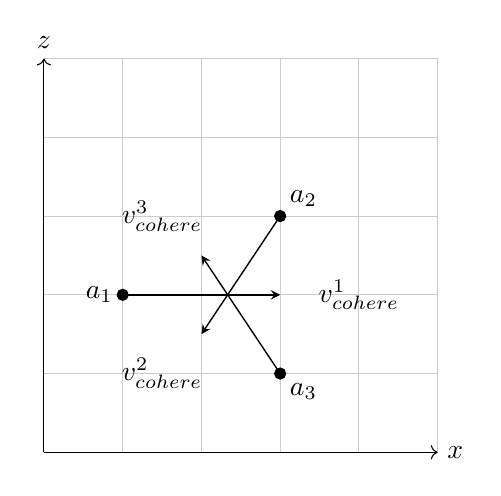
\begin{tikzpicture}
        \draw[thin,gray!40] (0,0) grid (5,5);
        \draw[->] (0,0)--(5,0) node[right]{$x$};
        \draw[->] (0,0)--(0,5) node[above]{$z$};

        \filldraw[black] (1,2) circle (2pt) node[anchor=east]{$a_1$};
        \filldraw[black] (3,3) circle (2pt) node[anchor=south west]{$a_2$};
        \filldraw[black] (3,1) circle (2pt) node[anchor=north west]{$a_3$};

        \draw[line width=0.5pt,black,-stealth](1,2)--(3,2) node at (4,2){$v^1_{cohere}$};
        \draw[line width=0.5pt,black,-stealth](3,3)--(2,1.5) node at (1.5,1){$v^2_{cohere}$};
        \draw[line width=0.5pt,black,-stealth](3,1)--(2,2.5) node at (1.5,3){$v^3_{cohere}$};
        
      \end{tikzpicture}
    \caption{Alignment vectors for three nearby agents}
    \label{fig:cohesion-2d}
\end{figure}

\subsubsection{Combining Behaviours}
\label{sec:combining-behaviours}

Fig. \ref{fig:cohesion-2d} demonstrates that the balance between cohesion and separation is important. If the cohesion force is too strong, the agents will collide, as shown. If the separation force is too strong, the agents will become disconnected and fly apart. This is similar in principle to the \emph{strong nuclear force} acting within the nucleus of an atom. The force is repulsive at close ranges (the avoidance radius), but attractive at larger ranges (the neighbourhood). We will explore this further in Section \ref{sec:lpfe}.

In general, tuning the influence of all three components is challenging. Even considering the constants in the simulation, \citet{Reynolds} notes that the relative weights that influence the strength of each component `\emph{is a precarious interrelationship that is difficult to adjust}'. Despite this, we can combine these three independent behaviours and attempt to tune them. 

We can define a \emph{composite behaviour}, which is defined as a linear combination of weights and behaviour vectors. In three dimensions, for the three behaviours, we have:

\begin{equation}
    \vec{V} = \alpha
    \begin{bmatrix}
    x_{avoid} \\
    y_{avoid} \\
    z_{avoid}
    \end{bmatrix}
    +
    \beta
    \begin{bmatrix}
    x_{align} \\
    y_{align} \\
    z_{align}
    \end{bmatrix}
    +
    \gamma
    \begin{bmatrix}
    x_{cohere} \\
    y_{cohere} \\
    z_{cohere}
    \end{bmatrix}
\end{equation}

The method for tuning the constants $\alpha, \beta, \gamma$ is empirical; we can observe the behaviour of the agents and adjust the values accordingly. We introduce the method for this below.

Initially, we will set the constants as shown in Table \ref{tab:spawn-constants}. These may be adjusted later. Additionally, we will set the weights for each component as shown in Table \ref{tab:boids-weights}.

\begin{table}[h]
    \begin{minipage}{0.45\textwidth}
        \centering
        \begin{tabular}{| c | c |} 
        \hline
        Constant & Value \\ 
        \hline\hline
        Number of Agents & 8 \\
        \hline
        Spawn Radius & 4 \\
        \hline
        Neighbour Radius & 1 \\
        \hline
        Square Avoidance Radius & 16 \\
        \hline
        \end{tabular}
        \caption{Spawn Constants}
        \label{tab:spawn-constants}
    \end{minipage}
    \hfill
    \begin{minipage}{0.45\textwidth}
        \centering
        \begin{tabular}{| c | c |} 
        \hline
        Behaviour & Weight \\ 
        \hline\hline
        Separation & 1 \\
        \hline
        Alignment & 1 \\
        \hline
        Cohesion & 1 \\
        \hline
        \end{tabular}
        \caption{Boids Weights}
        \label{tab:boids-weights}
    \end{minipage}
\end{table}

We can then simulate a run with these constants, culimating in the eight agents' X and Z positions within the space of 10 seconds, updated every 0.5 seconds. The spawn radius is also shown by the black circle. This is shown in Fig. \ref{fig:exp1}. When discussing the behaviour of individual agents, we will refer to them by their X-coordinate upon despawning at $t=10$, left to right. We see in Fig. \ref{fig:exp1} that the agents do move together, in a straight line, signifying that the alignment weight is initially well-tuned. However, we notice the behviour of Agents 5 and 6. These agents spawn outside of each other's neighbour radius, so will never make an effort to move towards each other. Additionally, the avoidance weight is not strong enough to pull them towards each other (as a result of being replused away from Agents 4 and 7, respectively). We will modify the neighbourhood radius to \textbf{3} and increase the weight of avoidance to \textbf{1.5}. This simulation results in the positions in Fig. \ref{fig:exp2}. 

\begin{figure}[H]
\centering
\begin{subfigure}{.4\textwidth}
\begin{tikzpicture}[trim axis left, trim axis right]
    \begin{axis}[
        xlabel=X,
        ylabel=Z,
        legend pos=outer north east,
        colormap/cool,
    ]

    \draw (axis cs:0,0) circle [blue, radius=4];


\addplot [scatter, surf, mark=*, x filter/.code={\IfStrEq{\thisrow{DroneID}}{Agent 0}{}{\def\pgfmathresult{}}{\def\pgfmathresult{}}},]
    table [x=X, y=Z, col sep=comma, point meta=\thisrow{Time}] {droneData.csv};

\addplot [scatter, surf, mark=*, x filter/.code={\IfStrEq{\thisrow{DroneID}}{Agent 1}{}{\def\pgfmathresult{}}{\def\pgfmathresult{}}},]
    table [x=X, y=Z, col sep=comma, point meta=\thisrow{Time}] {droneData.csv};

\addplot [scatter, surf, mark=*, x filter/.code={\IfStrEq{\thisrow{DroneID}}{Agent 2}{}{\def\pgfmathresult{}}{\def\pgfmathresult{}}},]
    table [x=X, y=Z, col sep=comma, point meta=\thisrow{Time}] {droneData.csv};

\addplot [scatter, surf, mark=*, x filter/.code={\IfStrEq{\thisrow{DroneID}}{Agent 3}{}{\def\pgfmathresult{}}{\def\pgfmathresult{}}},]
    table [x=X, y=Z, col sep=comma, point meta=\thisrow{Time}] {droneData.csv};

\addplot [scatter, surf, mark=*, x filter/.code={\IfStrEq{\thisrow{DroneID}}{Agent 4}{}{\def\pgfmathresult{}}{\def\pgfmathresult{}}},]
    table [x=X, y=Z, col sep=comma, point meta=\thisrow{Time}] {droneData.csv};

\addplot [scatter, surf, mark=*, x filter/.code={\IfStrEq{\thisrow{DroneID}}{Agent 5}{}{\def\pgfmathresult{}}{\def\pgfmathresult{}}},]
    table [x=X, y=Z, col sep=comma, point meta=\thisrow{Time}] {droneData.csv};

\addplot [scatter, surf, mark=*, x filter/.code={\IfStrEq{\thisrow{DroneID}}{Agent 6}{}{\def\pgfmathresult{}}{\def\pgfmathresult{}}},]
    table [x=X, y=Z, col sep=comma, point meta=\thisrow{Time}] {droneData.csv};

\addplot [scatter, surf, mark=*, x filter/.code={\IfStrEq{\thisrow{DroneID}}{Agent 7}{}{\def\pgfmathresult{}}{\def\pgfmathresult{}}},]
    table [x=X, y=Z, col sep=comma, point meta=\thisrow{Time}] {droneData.csv};
    
    \end{axis}
\end{tikzpicture}
\caption{Initial}
\label{fig:exp1}
\end{subfigure}
\hfill
\begin{subfigure}{.4\textwidth}
    \begin{tikzpicture}[trim axis left, trim axis right]
        \begin{axis}[
            xlabel=X,
            ylabel=Z,
            legend pos=outer north east,
            colormap/cool,
        ]
    
        \draw (axis cs:0,0) circle [blue, radius=4];
    
    
    \addplot [scatter, surf, mark=*, x filter/.code={\IfStrEq{\thisrow{DroneID}}{Agent 0}{}{\def\pgfmathresult{}}{\def\pgfmathresult{}}},]
        table [x=X, y=Z, col sep=comma, point meta=\thisrow{Time}] {drone2.csv};
    
    \addplot [scatter, surf, mark=*, x filter/.code={\IfStrEq{\thisrow{DroneID}}{Agent 1}{}{\def\pgfmathresult{}}{\def\pgfmathresult{}}},]
        table [x=X, y=Z, col sep=comma, point meta=\thisrow{Time}] {drone2.csv};
    
    \addplot [scatter, surf, mark=*, x filter/.code={\IfStrEq{\thisrow{DroneID}}{Agent 2}{}{\def\pgfmathresult{}}{\def\pgfmathresult{}}},]
        table [x=X, y=Z, col sep=comma, point meta=\thisrow{Time}] {drone2.csv};
    
    \addplot [scatter, surf, mark=*, x filter/.code={\IfStrEq{\thisrow{DroneID}}{Agent 3}{}{\def\pgfmathresult{}}{\def\pgfmathresult{}}},]
        table [x=X, y=Z, col sep=comma, point meta=\thisrow{Time}] {drone2.csv};
    
    \addplot [scatter, surf, mark=*, x filter/.code={\IfStrEq{\thisrow{DroneID}}{Agent 4}{}{\def\pgfmathresult{}}{\def\pgfmathresult{}}},]
        table [x=X, y=Z, col sep=comma, point meta=\thisrow{Time}] {drone2.csv};
    
    \addplot [scatter, surf, mark=*, x filter/.code={\IfStrEq{\thisrow{DroneID}}{Agent 5}{}{\def\pgfmathresult{}}{\def\pgfmathresult{}}},]
        table [x=X, y=Z, col sep=comma, point meta=\thisrow{Time}] {drone2.csv};
    
    \addplot [scatter, surf, mark=*, x filter/.code={\IfStrEq{\thisrow{DroneID}}{Agent 6}{}{\def\pgfmathresult{}}{\def\pgfmathresult{}}},]
        table [x=X, y=Z, col sep=comma, point meta=\thisrow{Time}] {drone2.csv};
    
    \addplot [scatter, surf, mark=*, x filter/.code={\IfStrEq{\thisrow{DroneID}}{Agent 7}{}{\def\pgfmathresult{}}{\def\pgfmathresult{}}},]
        table [x=X, y=Z, col sep=comma, point meta=\thisrow{Time}] {drone2.csv};
        
        \end{axis}
    \end{tikzpicture}
    \caption{Avoidance Tuning}
    \label{fig:exp2}
\end{subfigure}
\caption{Simulations}
\end{figure}

Note that the agents intially move away from each other - this is due to the increased effects of avoidance. We note, however, that Agents 1 and 2 do not appear to be pulled together, despite being within each other's neighbourhood. To mitigate this, we can increase the weight of cohesion to \textbf{1.4} and reduce the square avoidance radius to \textbf{12}. Finally, we can increase the weight of alignment slightly, to \textbf{1.2}, to reduce the effects of agents veering at the sides of the flock. This simulation results in the positions in Fig. \ref{fig:exp3}.

\begin{figure}[H]
    \centering
    \begin{tikzpicture}[trim axis left, trim axis right]
        \begin{axis}[
            xlabel=X,
            ylabel=Z,
            legend pos=outer north east,
            colormap/cool,
        ]
    
        \draw (axis cs:0,0) circle [blue, radius=4];
    
    
    \addplot [scatter, surf, mark=*, x filter/.code={\IfStrEq{\thisrow{DroneID}}{Agent 0}{}{\def\pgfmathresult{}}{\def\pgfmathresult{}}},]
        table [x=X, y=Z, col sep=comma, point meta=\thisrow{Time}] {drone3.csv};
    
    \addplot [scatter, surf, mark=*, x filter/.code={\IfStrEq{\thisrow{DroneID}}{Agent 1}{}{\def\pgfmathresult{}}{\def\pgfmathresult{}}},]
        table [x=X, y=Z, col sep=comma, point meta=\thisrow{Time}] {drone3.csv};
    
    \addplot [scatter, surf, mark=*, x filter/.code={\IfStrEq{\thisrow{DroneID}}{Agent 2}{}{\def\pgfmathresult{}}{\def\pgfmathresult{}}},]
        table [x=X, y=Z, col sep=comma, point meta=\thisrow{Time}] {drone3.csv};
    
    \addplot [scatter, surf, mark=*, x filter/.code={\IfStrEq{\thisrow{DroneID}}{Agent 3}{}{\def\pgfmathresult{}}{\def\pgfmathresult{}}},]
        table [x=X, y=Z, col sep=comma, point meta=\thisrow{Time}] {drone3.csv};
    
    \addplot [scatter, surf, mark=*, x filter/.code={\IfStrEq{\thisrow{DroneID}}{Agent 4}{}{\def\pgfmathresult{}}{\def\pgfmathresult{}}},]
        table [x=X, y=Z, col sep=comma, point meta=\thisrow{Time}] {drone3.csv};
    
    \addplot [scatter, surf, mark=*, x filter/.code={\IfStrEq{\thisrow{DroneID}}{Agent 5}{}{\def\pgfmathresult{}}{\def\pgfmathresult{}}},]
        table [x=X, y=Z, col sep=comma, point meta=\thisrow{Time}] {drone3.csv};
    
    \addplot [scatter, surf, mark=*, x filter/.code={\IfStrEq{\thisrow{DroneID}}{Agent 6}{}{\def\pgfmathresult{}}{\def\pgfmathresult{}}},]
        table [x=X, y=Z, col sep=comma, point meta=\thisrow{Time}] {drone3.csv};
    
    \addplot [scatter, surf, mark=*, x filter/.code={\IfStrEq{\thisrow{DroneID}}{Agent 7}{}{\def\pgfmathresult{}}{\def\pgfmathresult{}}},]
        table [x=X, y=Z, col sep=comma, point meta=\thisrow{Time}] {drone3.csv};
        
        \end{axis}
    \end{tikzpicture}
    \caption{Final Tuning}
    \label{fig:exp3}
\end{figure}

The results from each stage of the tuning process have their strengths; for our purposes, the final tuning is the most appropriate due to their responsiveness within the flock.

\subsection{Extended Boids}
We have implemented the three behaviours of the Boids algorithm. We can now extend this to include a fourth behaviour, \emph{goal seeking}. This will allow us to simulate the agents' ability to seek a goal position within the world. We will discuss the implementation of this below.

\subsubsection{Goal Seeking}
\label{sec:goal-seek}
We can implement the agents' ability to seek for a goal position in a similar method to the three behaviours Reynolds mentions. We can define a \emph{goal sphere}, with a given radius, centred around a random position in the world. We can then implement the \emph{seeking} behaviour to calculate the distance vector between the agent and the goal. 

Specifically, we have:

\begin{equation}
\vec{D} = \vec{g} - \vec{a}
\end{equation}

We can then apply a force vector in the direction of the goal. At present, we choose the weight of the seeking behaviour to be 2, so that it is most prominent. This results in some interesting `orbiting' behaviour. The location of the goal is shown by the green circle in Fig. \ref{fig:exp4}. We note that the agents do not actually enter the goal radius. This behaviour was likely down to the method being used before to implement the agent's moves. The agent would receive the given force vector, then normalise it - acting as a maximum clamping value for the force. This turned out to not be best practice, as whilst in close spaces, the direction of the desired goal \emph{(e.g. avoidance of nearby neighbours)} would be more important than the magnitude of the force, at higher distances between the current and goal position of the agent, the magnitudes, specifically of the pitch and roll components, become more significant in path planning. As an alternative, we simply use Unity's built in \verb|Math.Clamp| function to set the minimum and maximum foce values to ones we deem safe. An example simulation is seen below in Fig. \ref{fig:exp5}.

\begin{figure}[H]
\centering
\begin{subfigure}{.45\textwidth}
\begin{tikzpicture}[trim axis left, trim axis right]
    \begin{axis}[
        axis equal,
        xlabel=X,
        ylabel=Z,
        legend pos=outer north east,
        colormap/cool,
        width=1.2\textwidth
    ]


    \draw (axis cs:0,0) circle [radius=4];
    


\addplot [scatter, surf, mark=*, x filter/.code={\IfStrEq{\thisrow{DroneID}}{Agent 0}{}{\def\pgfmathresult{}}{\def\pgfmathresult{}}},]
    table [x=X, y=Z, col sep=comma, point meta=\thisrow{Time}] {drone4.csv};

\addplot [scatter, surf, mark=*, x filter/.code={\IfStrEq{\thisrow{DroneID}}{Agent 1}{}{\def\pgfmathresult{}}{\def\pgfmathresult{}}},]
    table [x=X, y=Z, col sep=comma, point meta=\thisrow{Time}] {drone4.csv};

\addplot [scatter, surf, mark=*, x filter/.code={\IfStrEq{\thisrow{DroneID}}{Agent 2}{}{\def\pgfmathresult{}}{\def\pgfmathresult{}}},]
    table [x=X, y=Z, col sep=comma, point meta=\thisrow{Time}] {drone4.csv};

\addplot [scatter, surf, mark=*, x filter/.code={\IfStrEq{\thisrow{DroneID}}{Agent 3}{}{\def\pgfmathresult{}}{\def\pgfmathresult{}}},]
    table [x=X, y=Z, col sep=comma, point meta=\thisrow{Time}] {drone4.csv};

\addplot [scatter, surf, mark=*, x filter/.code={\IfStrEq{\thisrow{DroneID}}{Agent 4}{}{\def\pgfmathresult{}}{\def\pgfmathresult{}}},]
    table [x=X, y=Z, col sep=comma, point meta=\thisrow{Time}] {drone4.csv};

\addplot [scatter, surf, mark=*, x filter/.code={\IfStrEq{\thisrow{DroneID}}{Agent 5}{}{\def\pgfmathresult{}}{\def\pgfmathresult{}}},]
    table [x=X, y=Z, col sep=comma, point meta=\thisrow{Time}] {drone4.csv};

\addplot [scatter, surf, mark=*, x filter/.code={\IfStrEq{\thisrow{DroneID}}{Agent 6}{}{\def\pgfmathresult{}}{\def\pgfmathresult{}}},]
    table [x=X, y=Z, col sep=comma, point meta=\thisrow{Time}] {drone4.csv};

\addplot [scatter, surf, mark=*, x filter/.code={\IfStrEq{\thisrow{DroneID}}{Agent 7}{}{\def\pgfmathresult{}}{\def\pgfmathresult{}}},]
    table [x=X, y=Z, col sep=comma, point meta=\thisrow{Time}] {drone4.csv};

    \draw [green, line width=0.7mm] (axis cs:-16,-29) circle [radius=3.45];
    
    \end{axis}
\end{tikzpicture}
\caption{Normalised Force Vector}
\label{fig:exp4}
\end{subfigure}
\hfill
\begin{subfigure}{.45\textwidth}
    \centering
    \begin{tikzpicture}[trim axis left, trim axis right]
        \begin{axis}[
            axis equal,
            xlabel=X,
            ylabel=Z,
            legend pos=outer north east,
            colormap/cool,
            width=1.2\textwidth
        ]
    
        \draw (axis cs:0,0) circle [radius=4];
    
    
    \addplot [scatter, surf, mark=*, x filter/.code={\IfStrEq{\thisrow{DroneID}}{Agent 0}{}{\def\pgfmathresult{}}{\def\pgfmathresult{}}},]
        table [x=X, y=Z, col sep=comma, point meta=\thisrow{Time}] {drone5.csv};
    
    \addplot [scatter, surf, mark=*, x filter/.code={\IfStrEq{\thisrow{DroneID}}{Agent 1}{}{\def\pgfmathresult{}}{\def\pgfmathresult{}}},]
        table [x=X, y=Z, col sep=comma, point meta=\thisrow{Time}] {drone5.csv};
    
    \addplot [scatter, surf, mark=*, x filter/.code={\IfStrEq{\thisrow{DroneID}}{Agent 2}{}{\def\pgfmathresult{}}{\def\pgfmathresult{}}},]
        table [x=X, y=Z, col sep=comma, point meta=\thisrow{Time}] {drone5.csv};
    
    \addplot [scatter, surf, mark=*, x filter/.code={\IfStrEq{\thisrow{DroneID}}{Agent 3}{}{\def\pgfmathresult{}}{\def\pgfmathresult{}}},]
        table [x=X, y=Z, col sep=comma, point meta=\thisrow{Time}] {drone5.csv};
    
    \addplot [scatter, surf, mark=*, x filter/.code={\IfStrEq{\thisrow{DroneID}}{Agent 4}{}{\def\pgfmathresult{}}{\def\pgfmathresult{}}},]
        table [x=X, y=Z, col sep=comma, point meta=\thisrow{Time}] {drone5.csv};
    
    \addplot [scatter, surf, mark=*, x filter/.code={\IfStrEq{\thisrow{DroneID}}{Agent 5}{}{\def\pgfmathresult{}}{\def\pgfmathresult{}}},]
        table [x=X, y=Z, col sep=comma, point meta=\thisrow{Time}] {drone5.csv};
    
    \addplot [scatter, surf, mark=*, x filter/.code={\IfStrEq{\thisrow{DroneID}}{Agent 6}{}{\def\pgfmathresult{}}{\def\pgfmathresult{}}},]
        table [x=X, y=Z, col sep=comma, point meta=\thisrow{Time}] {drone5.csv};
    
    \addplot [scatter, surf, mark=*, x filter/.code={\IfStrEq{\thisrow{DroneID}}{Agent 7}{}{\def\pgfmathresult{}}{\def\pgfmathresult{}}},]
        table [x=X, y=Z, col sep=comma, point meta=\thisrow{Time}] {drone5.csv};
    
    \draw [green, line width=0.7mm] (axis cs:27,22) circle [radius=3.45];

    \end{axis}
\end{tikzpicture}
\caption{Clamped Force Vector}
\label{fig:exp5}
\end{subfigure}
\caption{Seeking Behaviour}
\label{fig:exp45}
\end{figure}

The behaviour now seen in Fig. \ref{fig:exp5} is accurate, but not ideal, as the agents overshoot the goal and find themselves backtracking during pathfinding. This can be mitigated by implementing an Error Controller, using the fundamentals of control theory discussed in Section \ref{sec:stabilisation}. This is done by modifying the force vector such that it reduces with the distance between the agent and the goal position.

We can then instruct the agents to stop once they have detected that they are within the goal space. An example simulation of this is shown in Fig. \ref{fig:exp6}. We note that the agents gravitate towards the centre of the goal space. This is unwanted, as it does not make enough considerations for adjacent agents and their respective avoidance radii. At this point, we can then reintroduce our three initial behaviours and tune the influence of \emph{seeking} accordingly. an example simulation of this can be seen in

At this stage, we note an important flaw with our current model. The weights of the individual behaviours, ideally, should not stay constant throughout the duration of flight. For example, when the agents are far away from the goal, the seeking behaviour should be more prominent. However, when the agents are close to the goal, the agents should be more keen to avoid each other. We introduce alternative models in Section.

\begin{figure}[H]
    \centering
    \begin{subfigure}{.45\textwidth}
    \begin{tikzpicture}[trim axis left, trim axis right]
        \begin{axis}[
            axis equal,
            xlabel=X,
            ylabel=Z,
            legend pos=outer north east,
            colormap/cool,
            width=1.2\textwidth
        ]
    
        \draw (axis cs:0,0) circle [radius=4];
    
    
    \addplot [scatter, surf, mark=*, x filter/.code={\IfStrEq{\thisrow{DroneID}}{Agent 0}{}{\def\pgfmathresult{}}{\def\pgfmathresult{}}},]
        table [x=X, y=Z, col sep=comma, point meta=\thisrow{Time}] {drone6.csv};
    
    \addplot [scatter, surf, mark=*, x filter/.code={\IfStrEq{\thisrow{DroneID}}{Agent 1}{}{\def\pgfmathresult{}}{\def\pgfmathresult{}}},]
        table [x=X, y=Z, col sep=comma, point meta=\thisrow{Time}] {drone6.csv};
    
    \addplot [scatter, surf, mark=*, x filter/.code={\IfStrEq{\thisrow{DroneID}}{Agent 2}{}{\def\pgfmathresult{}}{\def\pgfmathresult{}}},]
        table [x=X, y=Z, col sep=comma, point meta=\thisrow{Time}] {drone6.csv};
    
    \addplot [scatter, surf, mark=*, x filter/.code={\IfStrEq{\thisrow{DroneID}}{Agent 3}{}{\def\pgfmathresult{}}{\def\pgfmathresult{}}},]
        table [x=X, y=Z, col sep=comma, point meta=\thisrow{Time}] {drone6.csv};
    
    \addplot [scatter, surf, mark=*, x filter/.code={\IfStrEq{\thisrow{DroneID}}{Agent 4}{}{\def\pgfmathresult{}}{\def\pgfmathresult{}}},]
        table [x=X, y=Z, col sep=comma, point meta=\thisrow{Time}] {drone6.csv};
    
    \addplot [scatter, surf, mark=*, x filter/.code={\IfStrEq{\thisrow{DroneID}}{Agent 5}{}{\def\pgfmathresult{}}{\def\pgfmathresult{}}},]
        table [x=X, y=Z, col sep=comma, point meta=\thisrow{Time}] {drone6.csv};
    
    \addplot [scatter, surf, mark=*, x filter/.code={\IfStrEq{\thisrow{DroneID}}{Agent 6}{}{\def\pgfmathresult{}}{\def\pgfmathresult{}}},]
        table [x=X, y=Z, col sep=comma, point meta=\thisrow{Time}] {drone6.csv};
    
    \addplot [scatter, surf, mark=*, x filter/.code={\IfStrEq{\thisrow{DroneID}}{Agent 7}{}{\def\pgfmathresult{}}{\def\pgfmathresult{}}},]
        table [x=X, y=Z, col sep=comma, point meta=\thisrow{Time}] {drone6.csv};
    
    \draw [green, line width=0.7mm] (axis cs:21,-19) circle [radius=3.45];

    \end{axis}
\end{tikzpicture}
\caption{Final Seeking Behaviour}
\label{fig:exp6}
\end{subfigure}
\hfill
\begin{subfigure}{.45\textwidth}
    \centering
    \begin{tikzpicture}[trim axis left, trim axis right]
        \begin{axis}[
            axis equal,
            xlabel=X,
            ylabel=Z,
            legend pos=outer north east,
            colormap/cool,
            width=1.2\textwidth
        ]
    
        \draw (axis cs:0,0) circle [radius=4];
    
    
    \addplot [scatter, surf, mark=*, x filter/.code={\IfStrEq{\thisrow{DroneID}}{Agent 0}{}{\def\pgfmathresult{}}{\def\pgfmathresult{}}},]
        table [x=X, y=Z, col sep=comma, point meta=\thisrow{Time}] {drone7.csv};
    
    \addplot [scatter, surf, mark=*, x filter/.code={\IfStrEq{\thisrow{DroneID}}{Agent 1}{}{\def\pgfmathresult{}}{\def\pgfmathresult{}}},]
        table [x=X, y=Z, col sep=comma, point meta=\thisrow{Time}] {drone7.csv};
    
    \addplot [scatter, surf, mark=*, x filter/.code={\IfStrEq{\thisrow{DroneID}}{Agent 2}{}{\def\pgfmathresult{}}{\def\pgfmathresult{}}},]
        table [x=X, y=Z, col sep=comma, point meta=\thisrow{Time}] {drone7.csv};
    
    \addplot [scatter, surf, mark=*, x filter/.code={\IfStrEq{\thisrow{DroneID}}{Agent 3}{}{\def\pgfmathresult{}}{\def\pgfmathresult{}}},]
        table [x=X, y=Z, col sep=comma, point meta=\thisrow{Time}] {drone7.csv};
    
    \addplot [scatter, surf, mark=*, x filter/.code={\IfStrEq{\thisrow{DroneID}}{Agent 4}{}{\def\pgfmathresult{}}{\def\pgfmathresult{}}},]
        table [x=X, y=Z, col sep=comma, point meta=\thisrow{Time}] {drone7.csv};
    
    \addplot [scatter, surf, mark=*, x filter/.code={\IfStrEq{\thisrow{DroneID}}{Agent 5}{}{\def\pgfmathresult{}}{\def\pgfmathresult{}}},]
        table [x=X, y=Z, col sep=comma, point meta=\thisrow{Time}] {drone7.csv};
    
    \addplot [scatter, surf, mark=*, x filter/.code={\IfStrEq{\thisrow{DroneID}}{Agent 6}{}{\def\pgfmathresult{}}{\def\pgfmathresult{}}},]
        table [x=X, y=Z, col sep=comma, point meta=\thisrow{Time}] {drone7.csv};
    
    \addplot [scatter, surf, mark=*, x filter/.code={\IfStrEq{\thisrow{DroneID}}{Agent 7}{}{\def\pgfmathresult{}}{\def\pgfmathresult{}}},]
        table [x=X, y=Z, col sep=comma, point meta=\thisrow{Time}] {drone7.csv};
    
    \draw [green, line width=0.7mm] (axis cs:-29,12) circle [radius=3.45];

    \end{axis}
\end{tikzpicture}
\caption{Three Initial Behaviours + Seeking}
\label{fig:exp7}
\end{subfigure}
\caption{Finalising Seeking Behaviour}
\label{fig:exp67}
\end{figure}

\subsubsection{Terrain Generation}
In previous sections, we have focused on the pathfinding behaviour of the agents in an empty space. However, in the real world, there are many obstacles that the agents must avoid. In this section, we introduce a terrain model to the simulation to parallel real world deviations in terrain heights. This is done using Perlin Noise\cite[289-293]{Perlin}. Specifically, for our implementation, we will look at generating a waveform with frequency $f$ and amplitude $A$ to model the terrain. We can then use this waveform to generate a heightmap for our terrain mesh.

We will consider four parameters which characterise how our terrain is generated. The number of octaves, $O_n$, lacunarity, $l$, persistence, $p$, and scale, $s$.
An octave is a measure of the ratio bewteen frequencies in a waveform. Accordingly, the lacunarity, $l$, controls the increase in frequency between octaves; an increase in lacunarity results in an increase in frequency between octaves. This is characterised by the realtionship:

$$\forall x \in \{O_1,O_2,...,O_n\}, f_x = l^{O_x}$$

Lacunarity, then, allows us to tune the increase in detail between octaves. We can see in Fig. \ref{fig:lacunarity}, with four octaves, the effect of lacunarity on the generated terrain. We can see that as the lacunarity increases, the terrain becomes more `spiky'.

\begin{figure}[H]
    \centering
    \begin{subfigure}{0.3\textwidth}
        \centering
        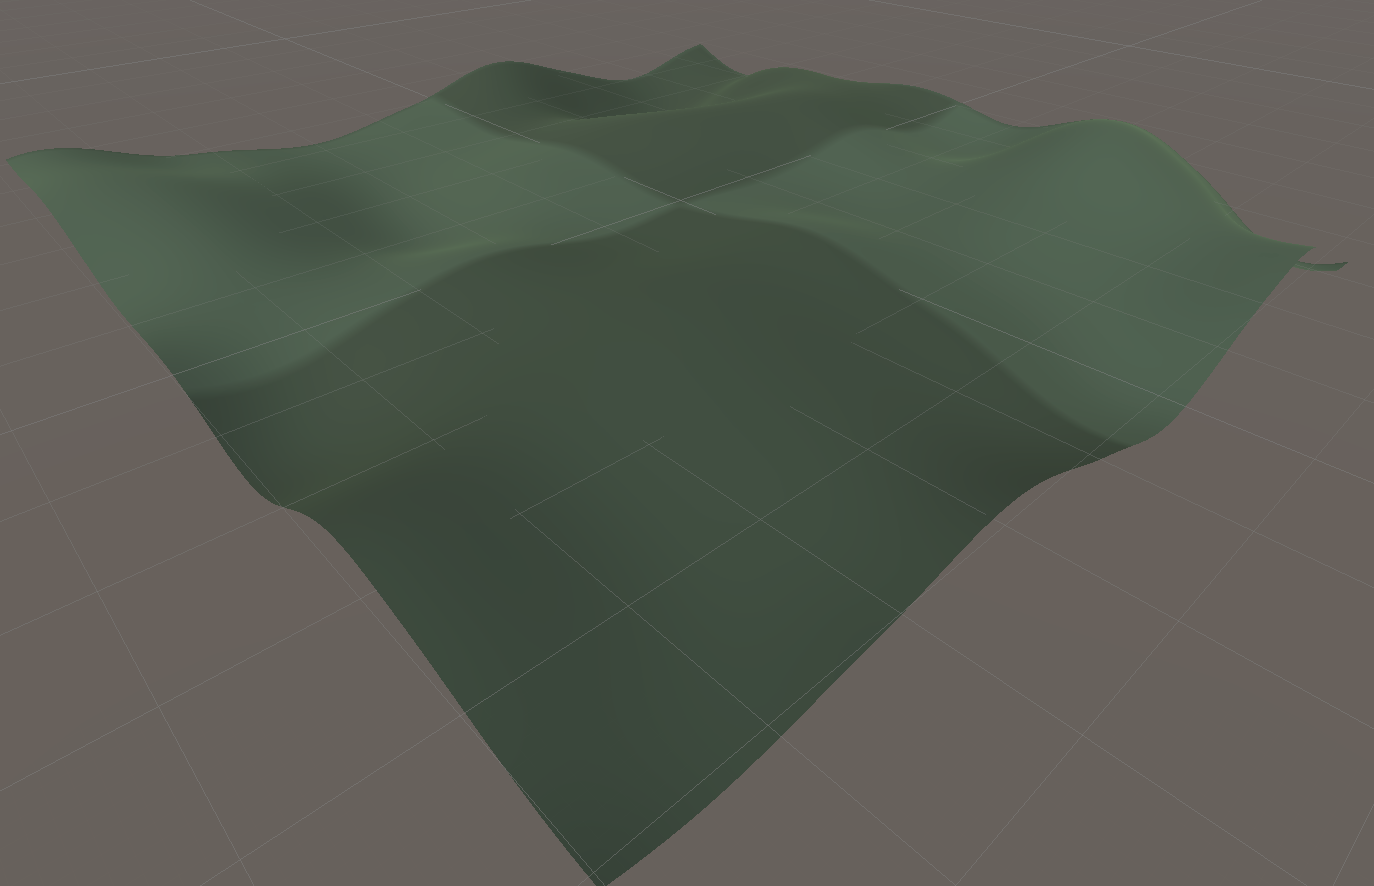
\includegraphics[width=\linewidth]{lacunarity1.png}
        \caption{$l=1$}
        \label{fig:lacunarity1}
    \end{subfigure}
    \hfill
    \begin{subfigure}{0.3\textwidth}
        \centering
        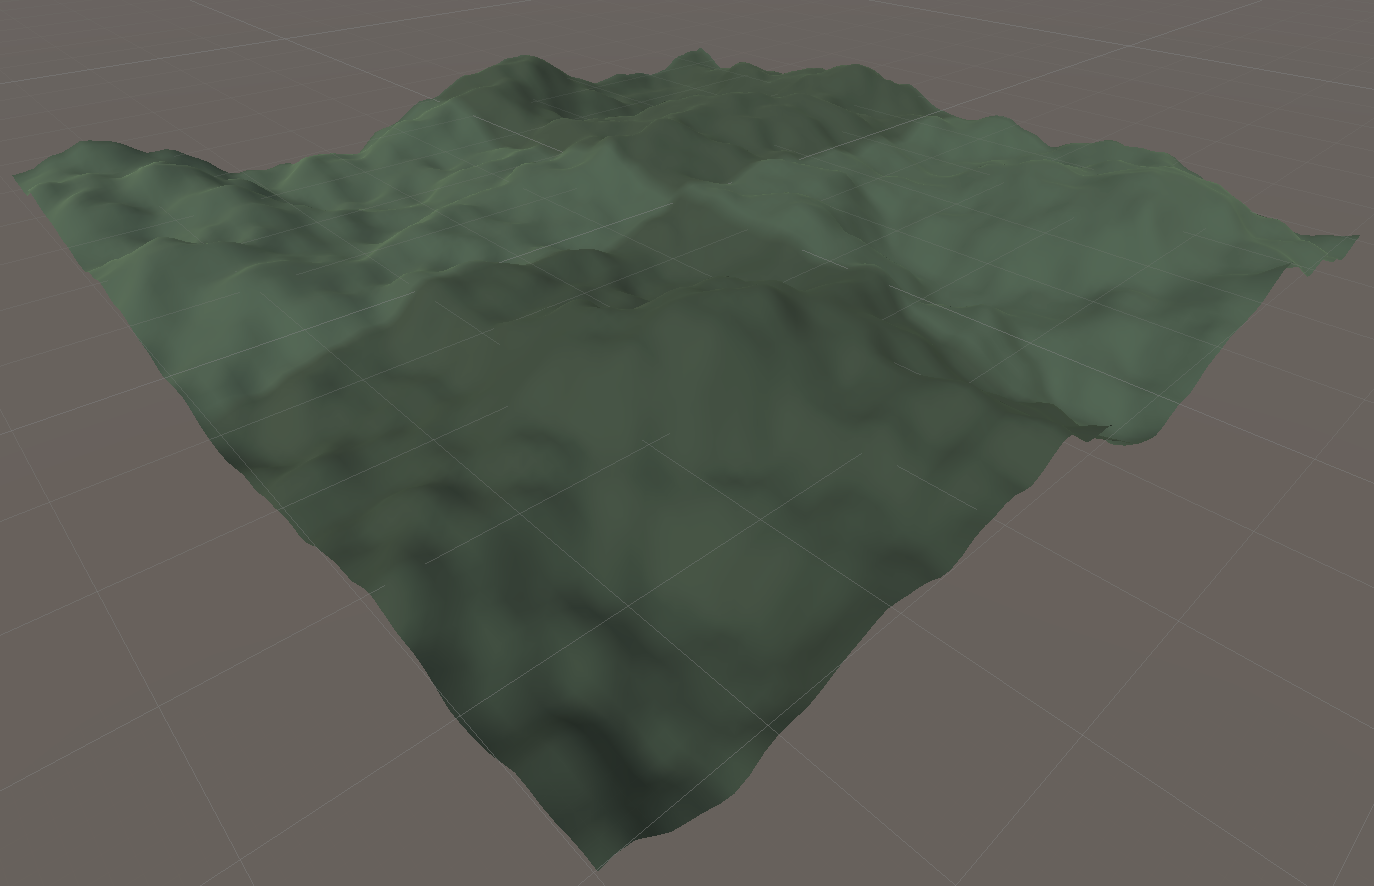
\includegraphics[width=\linewidth]{lacunarity2.png}
        \caption{$l=2$}
        \label{fig:lacunarity2}
    \end{subfigure}
    \hfill
    \begin{subfigure}{0.3\textwidth}
        \centering
        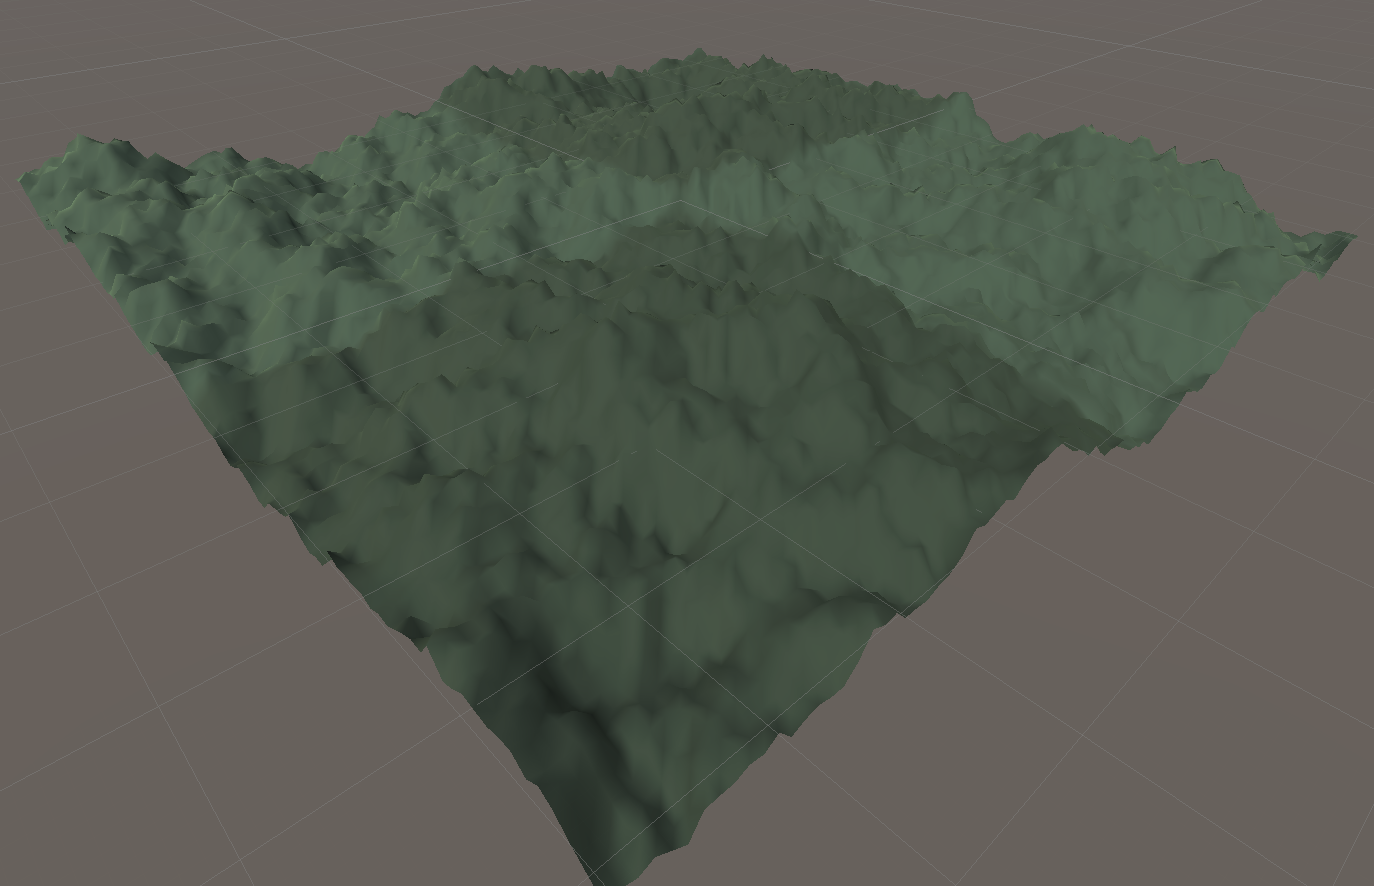
\includegraphics[width=\linewidth]{lacunarity4.png}
        \caption{$l=4$}
        \label{fig:lacunarity4}
    \end{subfigure}
    \caption{The effect of lacunarity on the generated terrain}
    \label{fig:lacunarity}
\end{figure}


The persistence, $p$, controls the decrease in amplitude between octaves. This allows us to tune how much each subsequent octave decreases in contribution to the overall waveform. This is characterised by the relationship:

$$\forall x \in \{O_1,O_2,...,O_n\}, A_x = p^{O_x}$$

We can see below, in Fig. \ref{fig:persistence}, the effect of persistence on the generated terrain. We can see that as the persistence increases, the height of the smaller details in the terrain increases. As we have kept the lacunarity constant, the spikes are not as evident as with Fig. \ref{fig:lacunarity4}.

\begin{figure}[H]
    \centering
    \begin{subfigure}{0.3\textwidth}
        \centering
        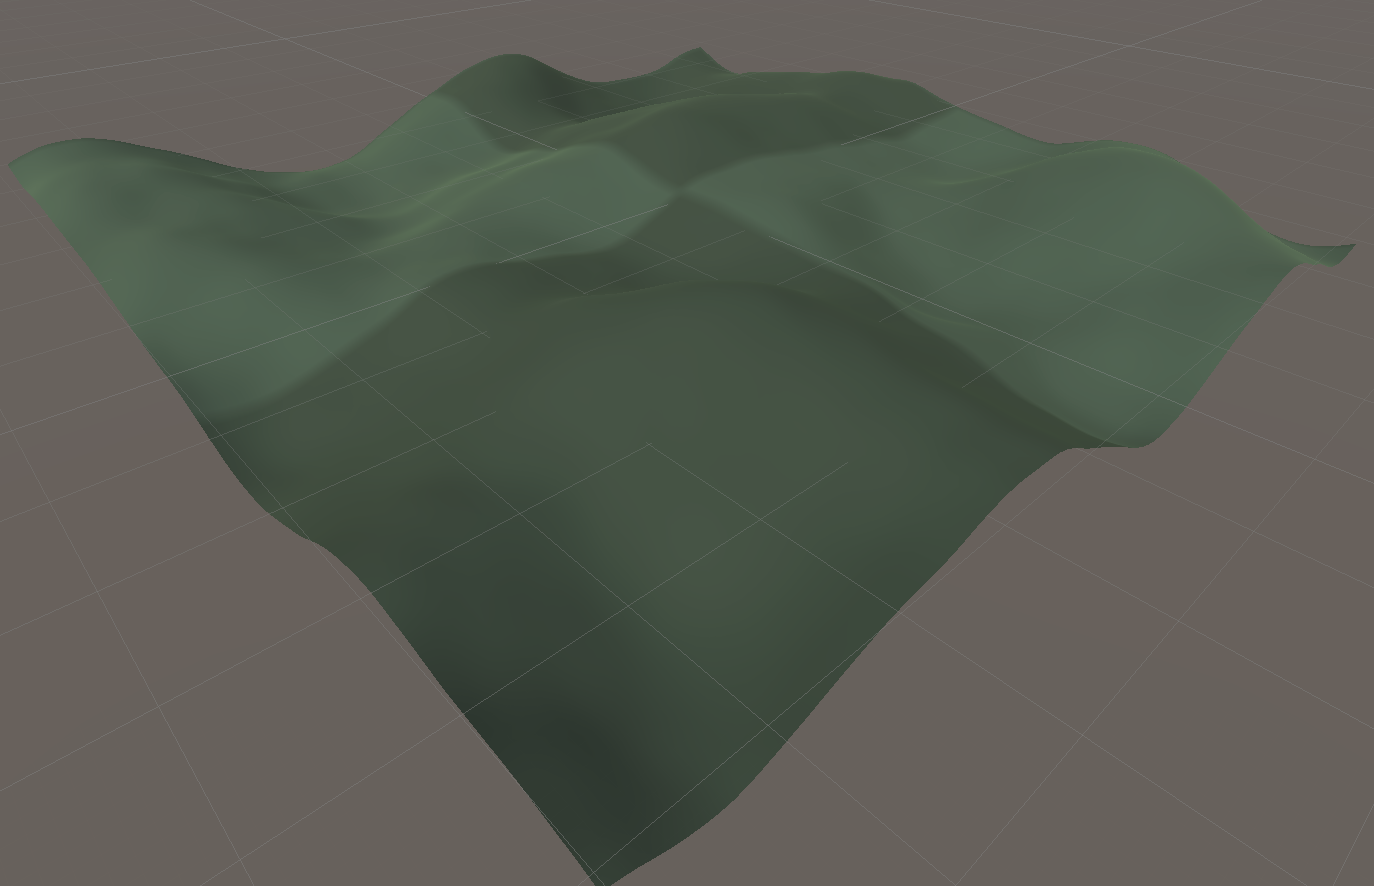
\includegraphics[width=\linewidth]{persistance0.2.png}
        \caption{$p=0.2$}
        \label{fig:persistence0.2}
    \end{subfigure}
    \hfill
    \begin{subfigure}{0.3\textwidth}
        \centering
        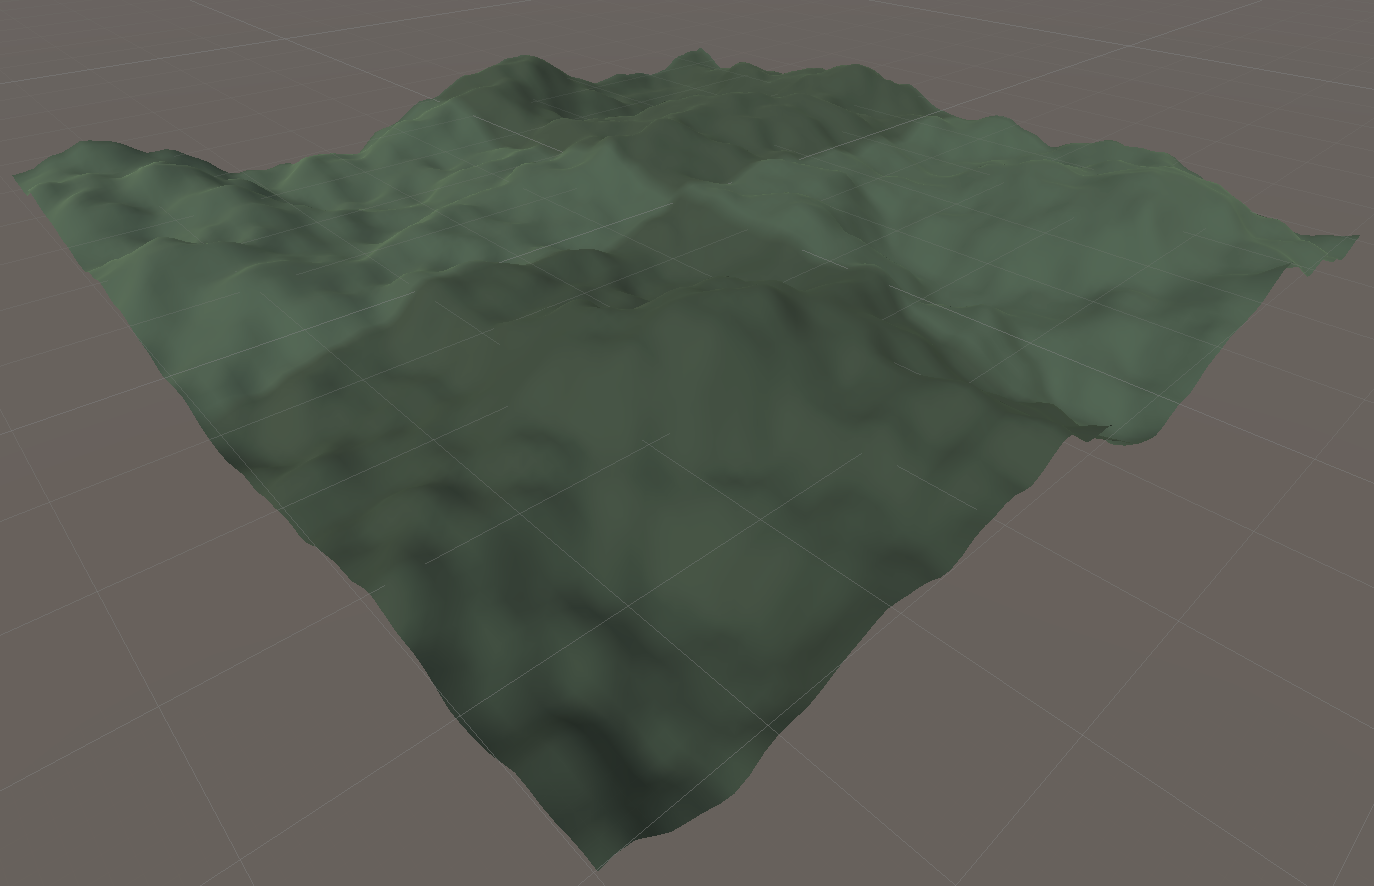
\includegraphics[width=\linewidth]{persistance0.5.png}
        \caption{$p=0.5$}
        \label{fig:persistence0.5}
    \end{subfigure}
    \hfill
    \begin{subfigure}{0.3\textwidth}
        \centering
        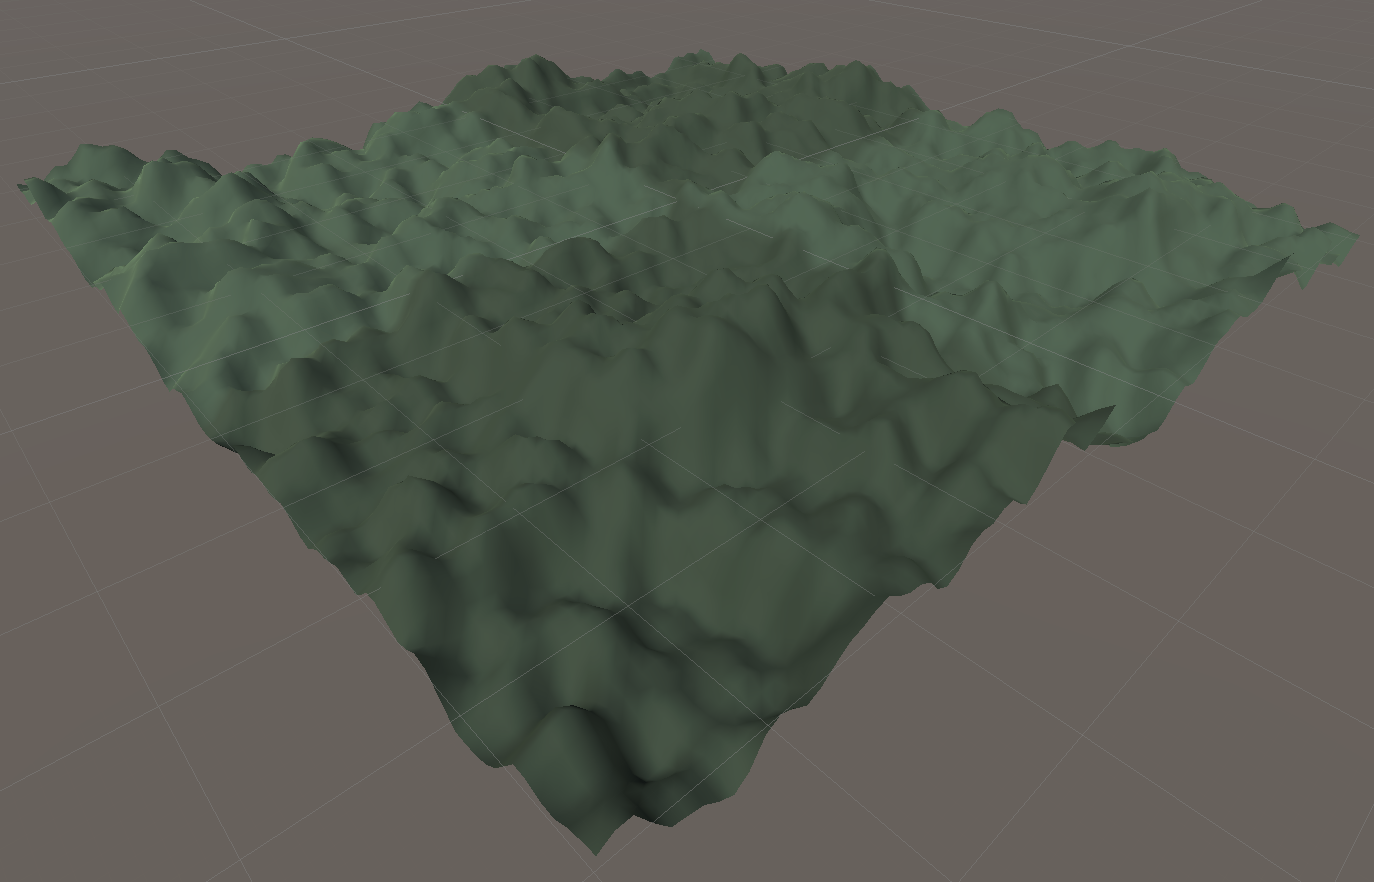
\includegraphics[width=\linewidth]{persistance0.8.png}
        \caption{$p=0.8$}
        \label{fig:persistence0.8}
    \end{subfigure}
    \caption{The effect of persistence on the generated terrain}
    \label{fig:persistence}
\end{figure}

Finally, the scale, $s$, contols the level of detail in the waveform that is applied to the terrain. We see in Fig. \ref{fig:scale}, the effect of scale on the generated terrain. We can see that as the scale increases, the terrain becomes more `zoomed out', and the details become less prominent. Notably, we can see a mountain ridge in the quadrant closest to the camera increase in size and distance away from the origin\footnote{The origin is the top left (the quadrant furthest away from the camera) of the terrain mesh.} between Fig. \ref{fig:scale25} and Fig. \ref{fig:scale28}.

\begin{figure}[H]
    \centering
    \begin{subfigure}{0.45\textwidth}
        \centering
        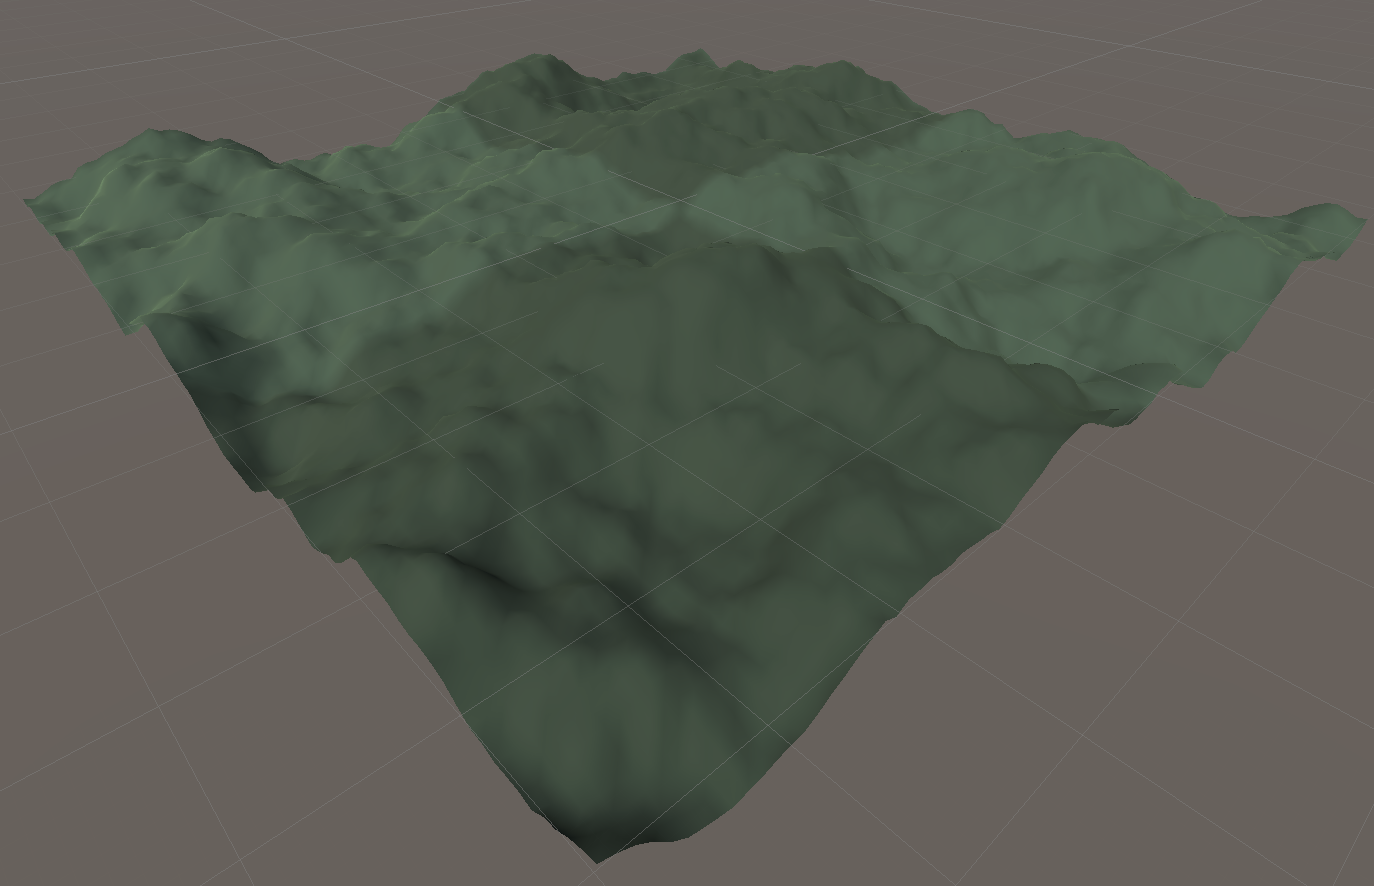
\includegraphics[width=\linewidth]{scale25.png}
        \caption{$s=25$}
        \label{fig:scale25}
    \end{subfigure}
    \hfill
    \begin{subfigure}{0.45\textwidth}
        \centering
        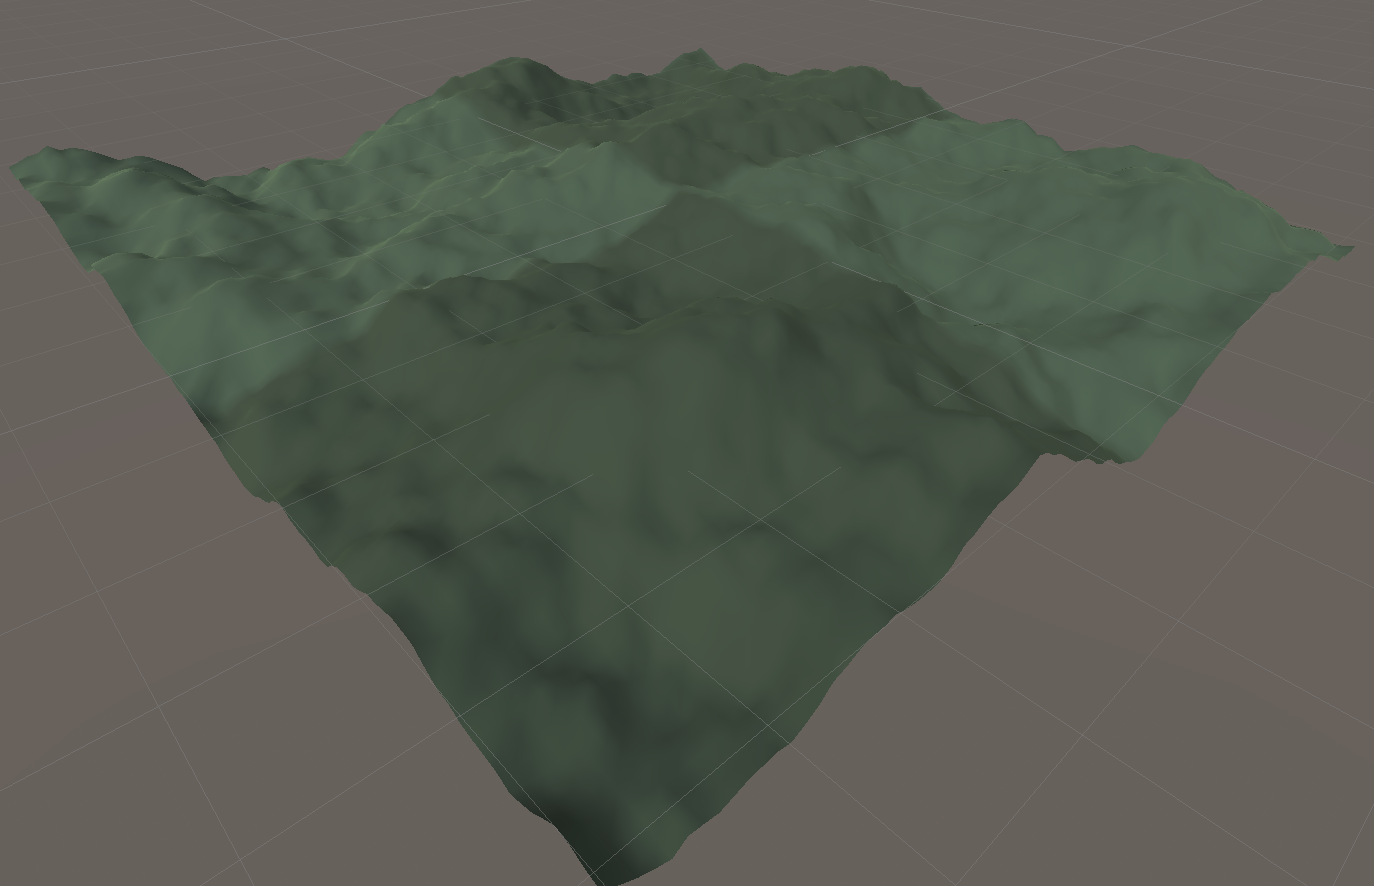
\includegraphics[width=\linewidth]{scale28.png}
        \caption{$s=28$}
        \label{fig:scale28}
    \end{subfigure}
    \caption{The effect of scale on the generated terrain}
    \label{fig:scale}
\end{figure}

After tuning the parameters based on a combination of empirical methods and noted examples \cite[pg.3-4]{Etherington}, the following parameters were chosen, with the final terrain mesh shown alongside:

\begin{figure}[ht]
    \centering
    \begin{subfigure}{0.4\textwidth}
        \centering
        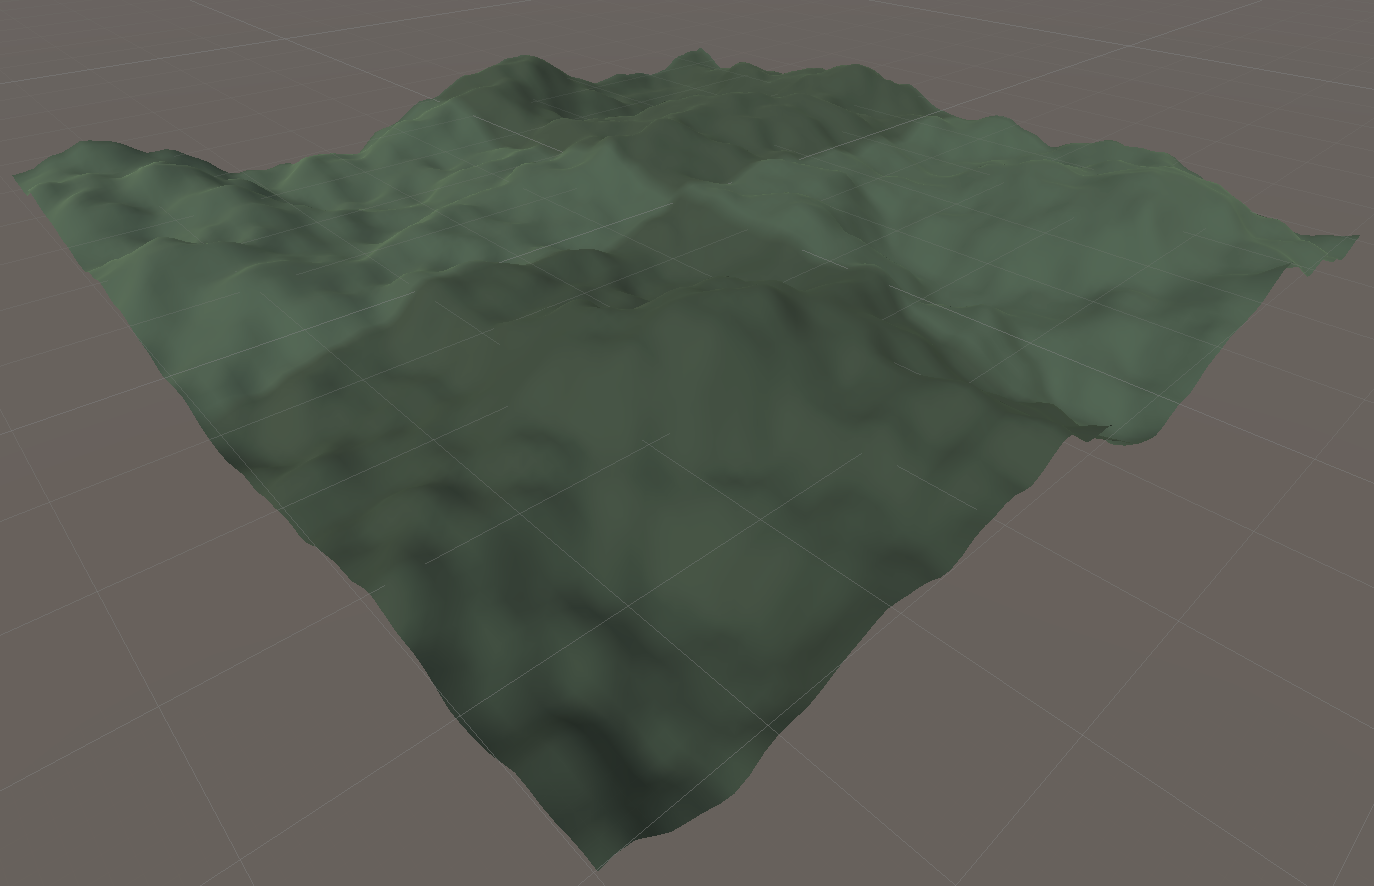
\includegraphics[width=\linewidth]{lacunarity2.png}
        \caption{Final Terrain Mesh}
        \label{fig:final}
    \end{subfigure}
    \hfill
    \begin{subfigure}{0.4\textwidth}
        \centering
        \begin{tabular}{|c|c|}
            \hline
            Parameter & Value \\
            \hline
            Number of Octaves & 4 \\
            \hline
            Lacunarity & 2 \\
            \hline
            Persistence & 0.5 \\
            \hline
            Scale & 25 \\
            \hline
        \end{tabular}
        \caption{Perlin Noise Parameter Values}
        \label{tab:parameter-values}
    \end{subfigure}
    \caption{}
    \label{fig:parameter-values-lacunarity2}
\end{figure}

\subsubsection{Terrain Avoidance}
\label{sec:terrain-avoidance}
Our final additional behaviour, then, will be to implement terrain avoidance. This will allow the agents to avoid the terrain mesh, and will be a crucial addition to the agents' autonomy. We will discuss the implementation of this below.

At present, we do not have a method to `sense' terrain. We can implement a simple method to detect terrain by casting a ray downwards from the agent's position, similar to a ranging sensor such as a LiDAR scanner.

We can then perform terrain avoidance by generating upward thrust, $u$ to cause an increase in the agent's local $y$ position, $a_y$ if the distance between the agent and the terrain is less than a given threshold, $t$. 

We can define this behaviour as follows:

\begin{equation}
    \vec{E} = \begin{bmatrix}
        0 \\
        U \\
        0
    \end{bmatrix}, U =
    \begin{cases}
        \vec{0} & \text{if } a_y > t \\
        u & \text{if } a_y \leq t
    \end{cases}
\end{equation}

We will initially set $t=5,u=10$.

We can see this behaviour in operation in Fig. \ref{fig:naive-ta-1}, where an agent approaches a steep hill. We see that before point 1, the agent does not increase its altitude. When a ray is cast at point 1, the agent detects that the distance between itself and the terrain is less than the threshold, and increases its altitude. Point 2 is the crest of the hill. At this point, the agent detects that there is still not enough distance between itself and the terrain, so the altitude continues to increase. In Fig. \ref{fig:naive-ta-2}, we see that the agent has detected the terrain, but appears to carry too much forward momentum and is locked in a tilt, so cannot avoid the hill.

\begin{figure}[H]
    \centering
    \begin{subfigure}{0.45\textwidth}
        \centering
        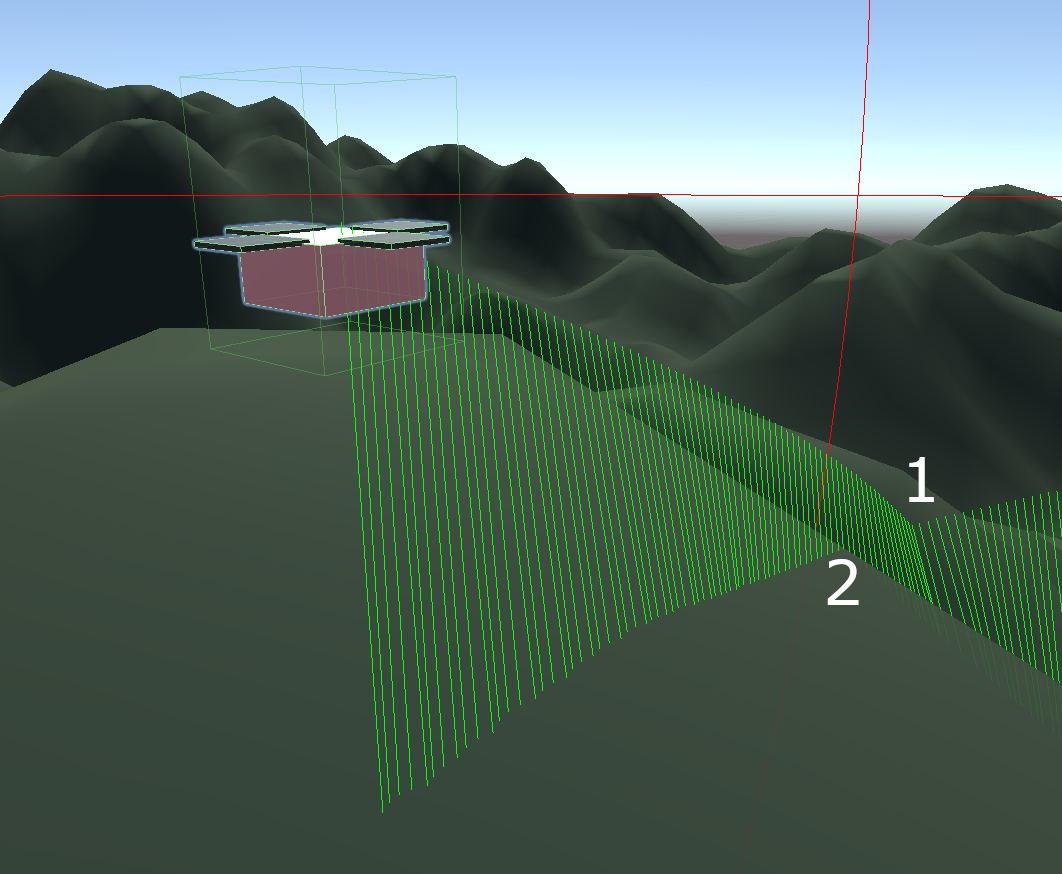
\includegraphics[width=\linewidth]{naive-ta-edited.png}
        \caption{Agent approaching a steep hill}
        \label{fig:naive-ta-1}
    \end{subfigure}
    \hfill
    \begin{subfigure}{0.45\textwidth}
        \centering
        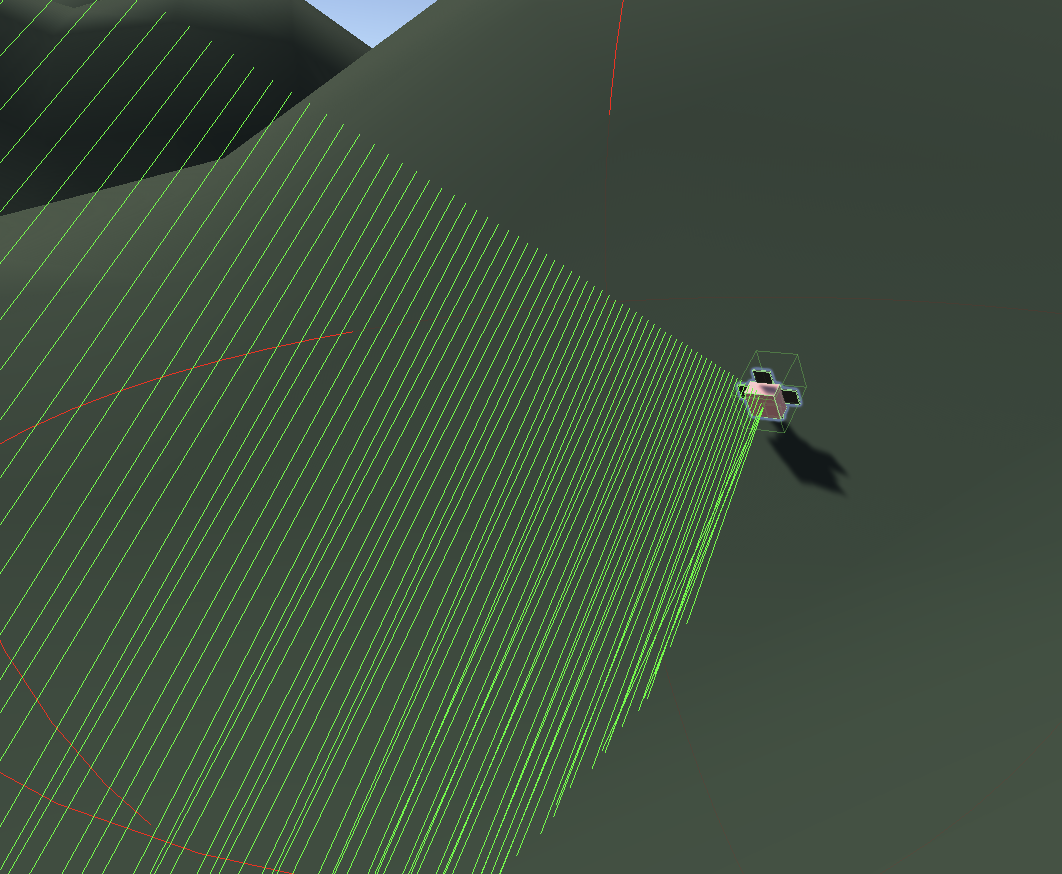
\includegraphics[width=\linewidth]{naive-ta-2.png}
        \caption{Agent failing to avoid terrain}
        \label{fig:naive-ta-2}
    \end{subfigure}
    \caption{Naive Terrain Avoidance}
    \label{fig:naive-ta-side-by-side}
\end{figure}

These observations indicate that the current implementation of terrain avoidance is not sufficient. We will modify our ranging sensor by tilting it slightly in the direction of the agent's velocity. This will allow the agent to detect the terrain in front of it, as well as below it, increasing the agent's ability to avoid terrain.

Unfortunately, the scale of the terrain proved a large challenge in optimising the avoidance behaviour. A limitation of the agents in the current implementation is that steep and large hills were hard to counter - mainly due to the behaviour only being able to avoid hills by increasing altitude. This is not ideal, as the agents should be able to avoid terrain by moving around it, rather than over it. We will discuss alternative methods in Section \ref{sec:lpfe}.

In line with the terrain changes, we will make some changes to how the simulation begins and ends. We define two platforms - a (red) start platform and a (green) end platform. The start platform is a flat surface, with a radius of 4, centred at the origin. The end platform is a flat surface, with a radius of 4, centred at a random point within a radius of 100m of the origin. The agents will begin on the start platform, and will be instructed to seek the end platform. These platforms are seen below in Fig. \ref{fig:platforms}.

\begin{figure}[H]
    \centering
    \begin{subfigure}{0.45\textwidth}
        \centering
        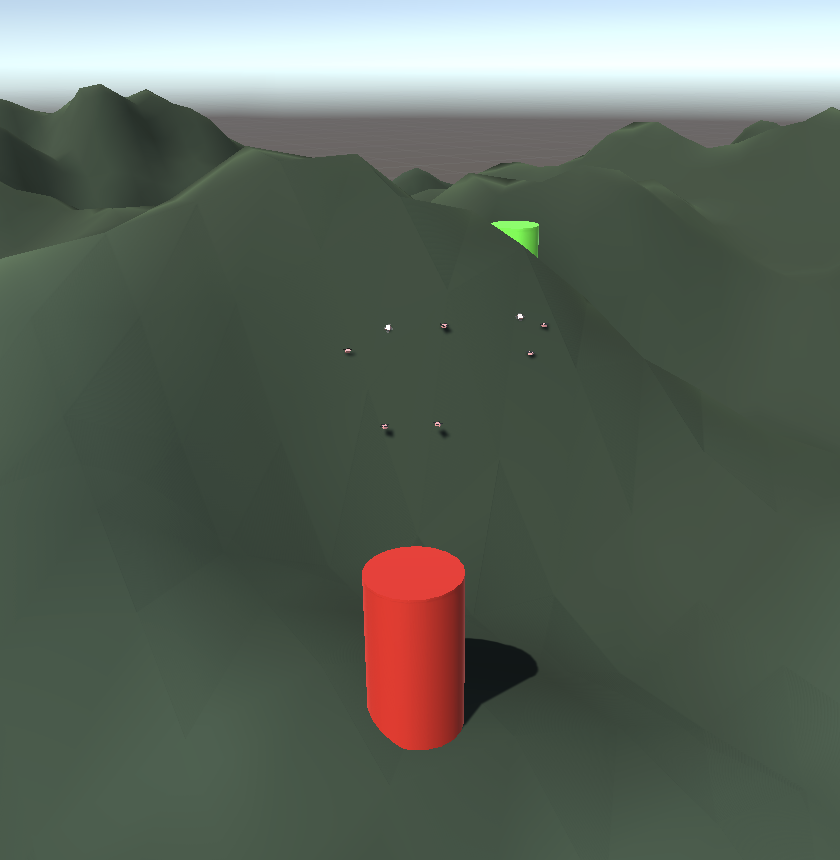
\includegraphics[width=\linewidth]{startplatform.png}
        \caption{Start Platform}
        \label{fig:startplatform}
    \end{subfigure}
    \hfill
    \begin{subfigure}{0.45\textwidth}
        \centering
        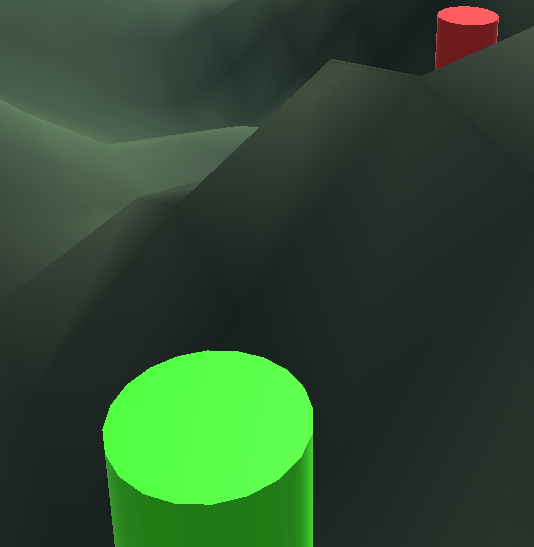
\includegraphics[width=\linewidth]{goalplatform.png}
        \caption{Goal Platform}
        \label{fig:goalplatform}
    \end{subfigure}
    \caption{Start and Goal Platforms in a single simulation}
    \label{fig:platforms}
\end{figure}

At this stage we have a set of behaviours that allow the agents to navigate a complex terrain mesh. We can now consider the optimisation of these behaviours to allow the agents to operate in a more autonomous manner.

\section{Methodology}
\label{sec:methodology}

In Section \ref{sec:introduction}, we discussed the desire to tailor the agent's behaviour to operate in particular scenarios, based on some expected applications of UAV swarms.

As such, we define three scenarios that we will aim to optimise the agent's behaviour for. Alongisde these scenarios, we will define some metrics that we will use to evaluate the agent's performance, which will be used to inform the cost function we aim to optimise.

\subsection{Scenario 1: Shortest First Arrival Time}
Firstly, we will consider the scenario where reaching the goal in the shortest time is the most important factor. This is a present requirement for time-sensitive situations, where the redundancy of multiple agents is used to ensure that the goal is reached as quickly as possible. In essence, it means agents can take more risks in their behaviour in order to achieve the objective.

Some example situations where this scenario would be of use include military operations in hostile environments, gaining situational awareness in disaster zones, and surveying hazardrous environments\cite{Srinath}.

For the simulations of this scenario, we will consider the following metrics:

\paragraph{First Arrival Time} 
We must consider the time taken for the first agent to reach the goal; it is the primary objective of the agents in this scenario. Specifically, this is the time taken for the first agent to enter the goal radius as defined in Section \ref{sec:goal-seek}. We define a simulation run time, which will be the length a simulation is allowed to run for.

For the purposes of normalisation, we will use the time taken for the first agent to reach the goal, divided by the simulation run time. This will give us a value between 0 and 1, where a lower number indicates a better performance.

This is the primary objective of the agents in this scenario, so we will give it a larger weighting in our cost function.

\paragraph{Proportion of Agents Arriving} A simulation run where more agents arrive at the goal is more successful than one where fewer agents arrive. Furthermore, a simulation run where no agents arrive would be considered a failure.

We will then, also consider the proportion of agents that do not arrive at the goal by the simulation run time. This will give us a value between 0 and 1, where a lower number indicates a better performance.

This is a secondary objective of the agents in this scenario.

\subsection{Scenario 2: Reduced Spread (Cohesivity)}
This scenario aims to reduce the spread of the agents in the flock. This is important in situations where the agents must maintain a close formation, such as in search and rescue operations, or in the delivery of goods. A simulation run's success in this scenario will be dependent on two metrics:

\paragraph{Standard Deviation of Arrival Times} We will consider the times at which the agents arrive at the goal, for all agents that arrive before the simulation run time. We will then calculate the standard deviation of these times. A lower standard deviation indicates that the agents are arriving at the goal in a more uniform manner. We will give this metric a larger weighting in our cost function.

A key issue with this metric is that it does not consider the method in which the agents arrive at the goal. For example, if all agents arrive at the goal at the same time, the standard deviation will be 0. This does not necessarily imply that the agents are in a close formation.

\paragraph{First Arrival Time} As with the first scenario, we still consider the time taken for the first agent to reach the goal. A run where all agents reach the goal with a low standard deviation between them, but taking a long time to do so is suboptimal. We will give this metric a smaller weighting in our cost function.

\paragraph{Proportion of Agents Arriving} As with the first scenario, we will consider the proportion of agents that do not arrive at the goal by the simulation run time. We do this to ensure that the cost function accounts for the number of agents within an arriving group.

\subsection{Scenario 3: Reducing Collision Numbers}
This scenario aims to reduce the number of collisions between agents and between agents and other objects in the environment. This is important in situations where the agents must operate in close proximity to each other, such as in the delivery of goods, or in the area monitoring. We will consider both the arrival time of the first agent and the proportion of agents that arrive at the goal, as in the previous scenarios, to a small extent, for similar reasons as justified previously.

We will also consider the following metrics: 

\paragraph{Number of Collisions} We will consider the number of collisions that occur between agents and between agents and objects in the environment. A simulation run where fewer collisions occur is more successful than one where more collisions occur. We will give this metric a larger weighting in our cost function.

\section{Optimisation}
Earlier, we utilised an empirical method to optimise our initial three behaviours. However, we note that for each extra parameter we introduce, the complexity of the parameter space increases exponentially. Consider an example in which each parameter is bounded by integers within the inclusive range $(0,10)$. With 3 parameters, this is a three dimensional parameter space with $11^3 = 1331$ possible combinations. With 5 parameters, this is a five dimensional parameter space with $11^5 = 161051$ possible combinations. This is a combinatorial explosion, and it is not feasible to optimise the parameters in this way.

Looking at other probabilistic methods for optimisation, two methods stand out. Firstly, genetic algorithms, which are inspired by the process of natural selection. This method is well researched within the field of behavioural optimisation in swarm robotics. One notable example is \citet{Alaliyat2014OptimisationOB}, who use a genetic algorithm for optimising the parameters of a Boids model. This is a computationally expensive method.

Alternatively, we may utilise a hill climbing\footnote{In this specific case, where we aim to minimise the cost function, this is more specifically a gradient descent algorithm.} algorithm. This is a simple optimisation algorithm that iteratively improves a solution by incrementally changing a single parameter. This method is less computationally expensive than a genetic algorithm, but it is also less likely to find the global minimum of a function, due to the likely presence of local minima, which the hill climbing algorithm cannot overcome.

Hence, we will look at an alternative method to find optimal values in the parameter space.

\subsection{Simulated Annealing}
The method we will use to optimise the parameters is simulated annealing. This is a probabilistic method that is used to find the global minimum of a function within a given search space. It is based on the physical process of annealing, where a material is heated and then cooled slowly to remove defects and reduce the material's energy. It is, in principle, a more advanced version of the hill climbing algorithm which can overcome local minima.

The algorithm works by starting at a random point in the search space. It then selects a random neighbour of the current point and evaluates the cost function at this point, $t$. If the cost function at the new point is lower than the cost function at the current point, the algorithm moves to the new point. If the cost function at the new point is higher than the cost function at the current point, the algorithm moves to the new point with a probability that is dependent on the difference between the cost function at the new point and the cost function at the current point,$|c(t) - c(t+1)|$ , and a temperature parameter, $T$. The algorithm then reduces the temperature parameter and repeats the process until the temperature parameter reaches a minimum value.

The method of which the temperature is reduced is crucial to the success of the algorithm. If the temperature is reduced too quickly, the algorithm may become stuck in a local minimum. If the temperature is reduced too slowly, the algorithm may take too long to converge to a solution. We will use a linear cooling schedule. That is, $T$ decreases linearly with each iteration of the algorithm.

We will define our acceptance function, $P \in (0,1)$ as follows:

\begin{equation}
    P = \begin{cases}
        1 & \text{if } c(t+1) < c(t) \\
        e^{-\frac{c(t+1) - c(t)}{T}} & \text{if } c(t+1) \geq c(t)
    \end{cases}
\end{equation}

We note the exponential term in the acceptance function. This is based on the \emph{Boltzmann distribution}, which is used in statistical mechanics to describe the probability of a system being in a certain state. The Boltzmann distribution is characterised by the equation:

\begin{equation}
    P(i) = e^{-\frac{E_i}{kT}}
\end{equation}

Given the Boltzmann constant, $k$, and the temperature, $T$, the probability of a system being in a state with energy $E_i$ is given by the above equation.

% more explanation needed here

We can then define our parameters and our cost function. As noted previously in Section \ref{sec:combining-behaviours}, the parameter space can be defined as a linear combination of the behaviours and their weights. For clarity, we now redifine this in terms of our extended parameter space, which includes the goal seeking and terrain avoidance behaviours.

\begin{equation}
\vec{V} = 
\alpha
\begin{bmatrix}
    x_{avoid} \\
    y_{avoid} \\
    z_{avoid} \\
\end{bmatrix}
+ \beta
\begin{bmatrix}
    x_{align} \\
    y_{align} \\
    z_{align} \\
\end{bmatrix}
+ \gamma
\begin{bmatrix}
    x_{cohere} \\
    y_{cohere} \\
    z_{cohere} \\
\end{bmatrix}
+ \delta
\begin{bmatrix}
    x_{seek} \\
    y_{seek} \\
    z_{seek} \\
\end{bmatrix}
+ \epsilon
\begin{bmatrix}
    x_{terrain} \\
    y_{terrain} \\
    z_{terrain} \\
\end{bmatrix}
\end{equation}

We can then define our cost function, which is a linear combination of the metrics defined in Section \ref{sec:methodology}. We will define a singular, modular cost function to allow for the easy addition of new metrics and the ability to tweak the weighting of the existing metrics. 

The cost function will normalise the given weights, and the given metrics will also be normalised to ensure the output of the cost function lies in the range $(0,1)$.

Specifically, we define the normalisation of the four weights as:
\begin{equation}
    \forall w_i \in W, w_i = \frac{w_i}{\sum_{i=0}^{|W|}{w_i}}
\end{equation}

We also define the normalised metrics as follows:

\paragraph{First Arrival Time}
We can normalise this value by dividing it by the simulation time (the length the simulation is allowed to run for).

Hence,
\begin{equation}
    m_1 = \frac{\text{firstArrivalTime}}{\text{simulationRuntime}}
\end{equation}

\paragraph{Proportion Reached}
In a similar nature to the normalisation method for the \emph{first arrival time} metric, we can divide the number of agents that have not reached the goal by the simulation time by the total number of agents in the simulation, namely:



% \begin{equation}
%     \begin{align}
%         \text{firstTime} &= \frac{\text{firstTime}}{\text{simulationTime}} \\
%         \text{proportionNotReached} &= \frac{\text{numOfAgents}-\text{numAgentsReached}}{\text{numOfAgents}} \\
%         % \text{standardDeviation} &= \frac{\text{standardDeviation}}{\text{simulationTime}} \\
%         % \text{collisionFactor} &= \frac{1}{1+e^{-0.1 * (collisionNumber - 40)}}
%     \end{align}
% \end{equation}


\subsection{Simulations}

\subsection{Results}


\section{Improving Autonomy}

\subsection{Boids (1999): Introducing Obstacle Avoidance}

\subsection{A Simplified Model}
We now aim to reduce the complexity of the parameter space in the hopes of strengthening the link between the parameters and the emergent behaviour.


\subsection{Local Potential Field Emergence}
\label{sec:lpfe}

\subsection{Final Results}




\section{Future Work}
\subsection{LPFE Implementation}

\subsection{Online Optimisation}

\subsection{Hostility}
\subsubsection{Hostile Environments}

\subsubsection{Hostile Agents}


\section{Evaluation}
\subsection{Project Management}

\subsection{Comparing Models}

\subsection{Speed-Success-Flock Size Tradeoffs}

\subsection{Use Cases}

\subsection{Author's Assessment of the Project}




\newpage
\bibliographystyle{IEEEtranN}
\bibliography{refs} 
\end{document}

